\documentclass[11pt]{article}
\usepackage[a4paper,left=22mm,right=22mm,top=23mm,bottom=25mm]{geometry}
\usepackage{graphicx}
\usepackage{url}
\usepackage{hyperref}
\usepackage{amsmath}
\usepackage{fancyhdr}
\usepackage[utf8]{inputenc}
\hypersetup{colorlinks=true,linkcolor=blue,urlcolor=blue}

\begin{document}
\clubpenalty 10000
\widowpenalty 10000

\title{4. Seznámení se se zvolenou pokročilou iterativní metodou na problému batohu}
\author{Ladislav Martínek}
\date{}
\maketitle
 
\section{Zadání úlohy} 

\begin{itemize}
\item Zvolte si heuristiku, kterou budete řešit problém vážené splnitelnosti booleovské formule (simulované ochlazování, simulovaná evoluce, tabu prohledávání)
\item Tuto heuristiku použijte pro řešení problému batohu. Můžete použít dostupné instance problému, anebo si vygenerujte své instance pomocí generátoru. Používejte instance s větším počtem věcí ($>$30).
\item Hlavním cílem domácí práce je seznámit se s danou heuristikou, zejména se způsobem, jakým se nastavují její parametry (rozvrh ochlazování, selekční tlak, tabu lhůta...) a modifikace (zjištění počáteční teploty, mechanismus slekce, tabu atributy...). Není-li Vám cokoli jasné, prosíme ptejte se na cvičeních.
\item Problém batohu není příliš obtížný, většinou budete mít k dispozici globální maxima (exaktní řešení) z předchozích prací, například z dynamického programování. Při správném nastavení parametrů byste měli vždy dosáhnout těchto optim, případně pouze velice malých chyb. Doba výpočtu může ovšem být relativně větší. Závěrečná úloha je co do nastavení a požadovaného výkonu heuristiky podstatně náročnější a může vyžadovat zcela jiné nastavení parametrů.

\end{itemize}


\section{Popis algoritmu simulovaného ochlazování}\label{kap:1}
Jako pokročilou heuristiku řešící problém batohu jsem si zvolil simulované ochlazování (někdy nazýváno simulované žíhání). Algoritmus je založen na simulovaném žíhání oceli. Pří žíhání ocely je teplota na počátku vysoká a vysoká je také kinetická energie částic. Teplota je postupně snižována a tím klesá i kinetická energie molekul a vazebné síly převáží a vznikají krystaly. Výsledná hmota je složena z krystalů, které se líši podle parametrů (např. rychlost ochlazování) tohoto procesu. 

Tedy anlogicky, vysoká teplota a energie představuje v systému vyšší pravděpodobnost přijetí horšího řešení při řešení problému batohu. Převažuje tedy princip explorace. S klesající teplotou již nechceme tolik přijímat zhoršující řešení a algoritmus spíš bude hleda optimum. Bude tedy převládat přincip exploatace, tedy prohledávání nejbližšího okolí a hledání optima. Pokud by jsme tento princip aplikovali od počátku mohlo by se stát, že by jsme brzo uvízly v lokálním minimu. 

Hlavní parametry algoritmu jsou tedy počáteční teplota, rychlost ochlazování a také počet iterací na jedné hodnotě teploty. Na počátku je tedy snaha prohlédávat větší okolí (diverzifikace), se snižující teplotou již změny nebudou tak veliké a algoritmus by měl dojít k nějakému lokálnímu optimu, které by mělo být nejlépe také globální (intenzifikace). 

Počateční teplota je snižována násobením koeficientem, který je typicky velmi blízko jedničce. V každé iteraci algoritmus generuje náhodně souseda, pro kterého lze jednoduše a rychle zjistit jeho kvalitu, pokud je lepší než současné, tak jej přijmu a pokračuji. Pokud je horší, tak jej s nějakou pravděpodobností přijmu také. Pravděpodobnost je závislá na teplotě. Příjímání je v algoritmu udělané tak, že generuji náhodné číslo od 0 do 1 a pokud je menší než hodnota $ e^{-(C(\text{nové řešení})-C(\text{aktuální řešení}))/teplota}$, tak řešení přijmu.

Poslední je třeba výřešit počátek algoritmu. Algoritmus může začínat například s prázdným batohem (využívám u svého řešení) nebo můžu obsah batohu generovat náhodně a žáčít tak s nhodně vyplňěným batohem.

\section{Experimenty}
Pro testování iterativní heuristiky jsem využil 100 instancí o velikosti 100 předmětů, u kterých znám optimální řešení a mohl jsem tedy počítat relativní chybu algoritmu mopocí vzorce $$\epsilon_{rel} = \frac{C(OPT)-C(APX)}{C(OPT)}$$. U řešení jsem generoval grafy pro vývoj řešení v závislosti na teplotě a měřil průměrnou chybu a čas.

Experimenty jsem prováděl v režimu jednoho vlákna na starším datovém serveru v podobě starého notebooku, který v době výpočtu nebyl používán. Výsledky tedy nejsou ovlivněny jinými běžícími programy. Procesor na testovacím stroji: \textit{Intel Pentium T3400 (2 cores). Taktován na 2.16~GHz s~1~MB cache}.
Měření času CPU probíhalo v knihovně $timeit$. Algoritmus jsem napsal v Cythonu a časy tedy nemohou být případně srovnávány s řešením v předchozích úlohách.

K závislostem na jednotlivých parametrech přídám ještě grafy vývoje řešení pro lepší vizualizaci závislosti a chování. Na grafu na ose X je teplota sestupně a na ose Y cena batohu. Na každém grafu je maximální dosažená cena a aktuální cena v algoritmu. Pro přehlednost této zprávy budou grafy zmenšené, ale nebude to mít vliv na názornost ukázky vývoje řešení. V plné velikosti jsou v přiloženém archivu, kde název je proměnný parametr a ostatní jsou zafixovány na hodnotách uvedených na grafu pro srovnání průměrné chyby a času.
 
\subsection{Cíle}

Vlastnosti algoritmu lze měnit pomocí parametrů, jako je počáteční teplota, ochlazování a počet iterací na jedné teplotě. Při řešení tohoto problému, jsem neuvažoval neplatná řešení, jelikož začínám s prázdným batohem. Cílem je otestovat chování algoritmu v závislosti na těchto parametrech a vyvodit závěry. Tedy se naučit iterativní heuristiku nastavit na tento problém a ředit ho pomocí ní. 


\subsection{Závislost na počáteční teplotě}
\begin{figure}
	\centering
    \begin{minipage}[c]{0.49\textwidth}
        \centering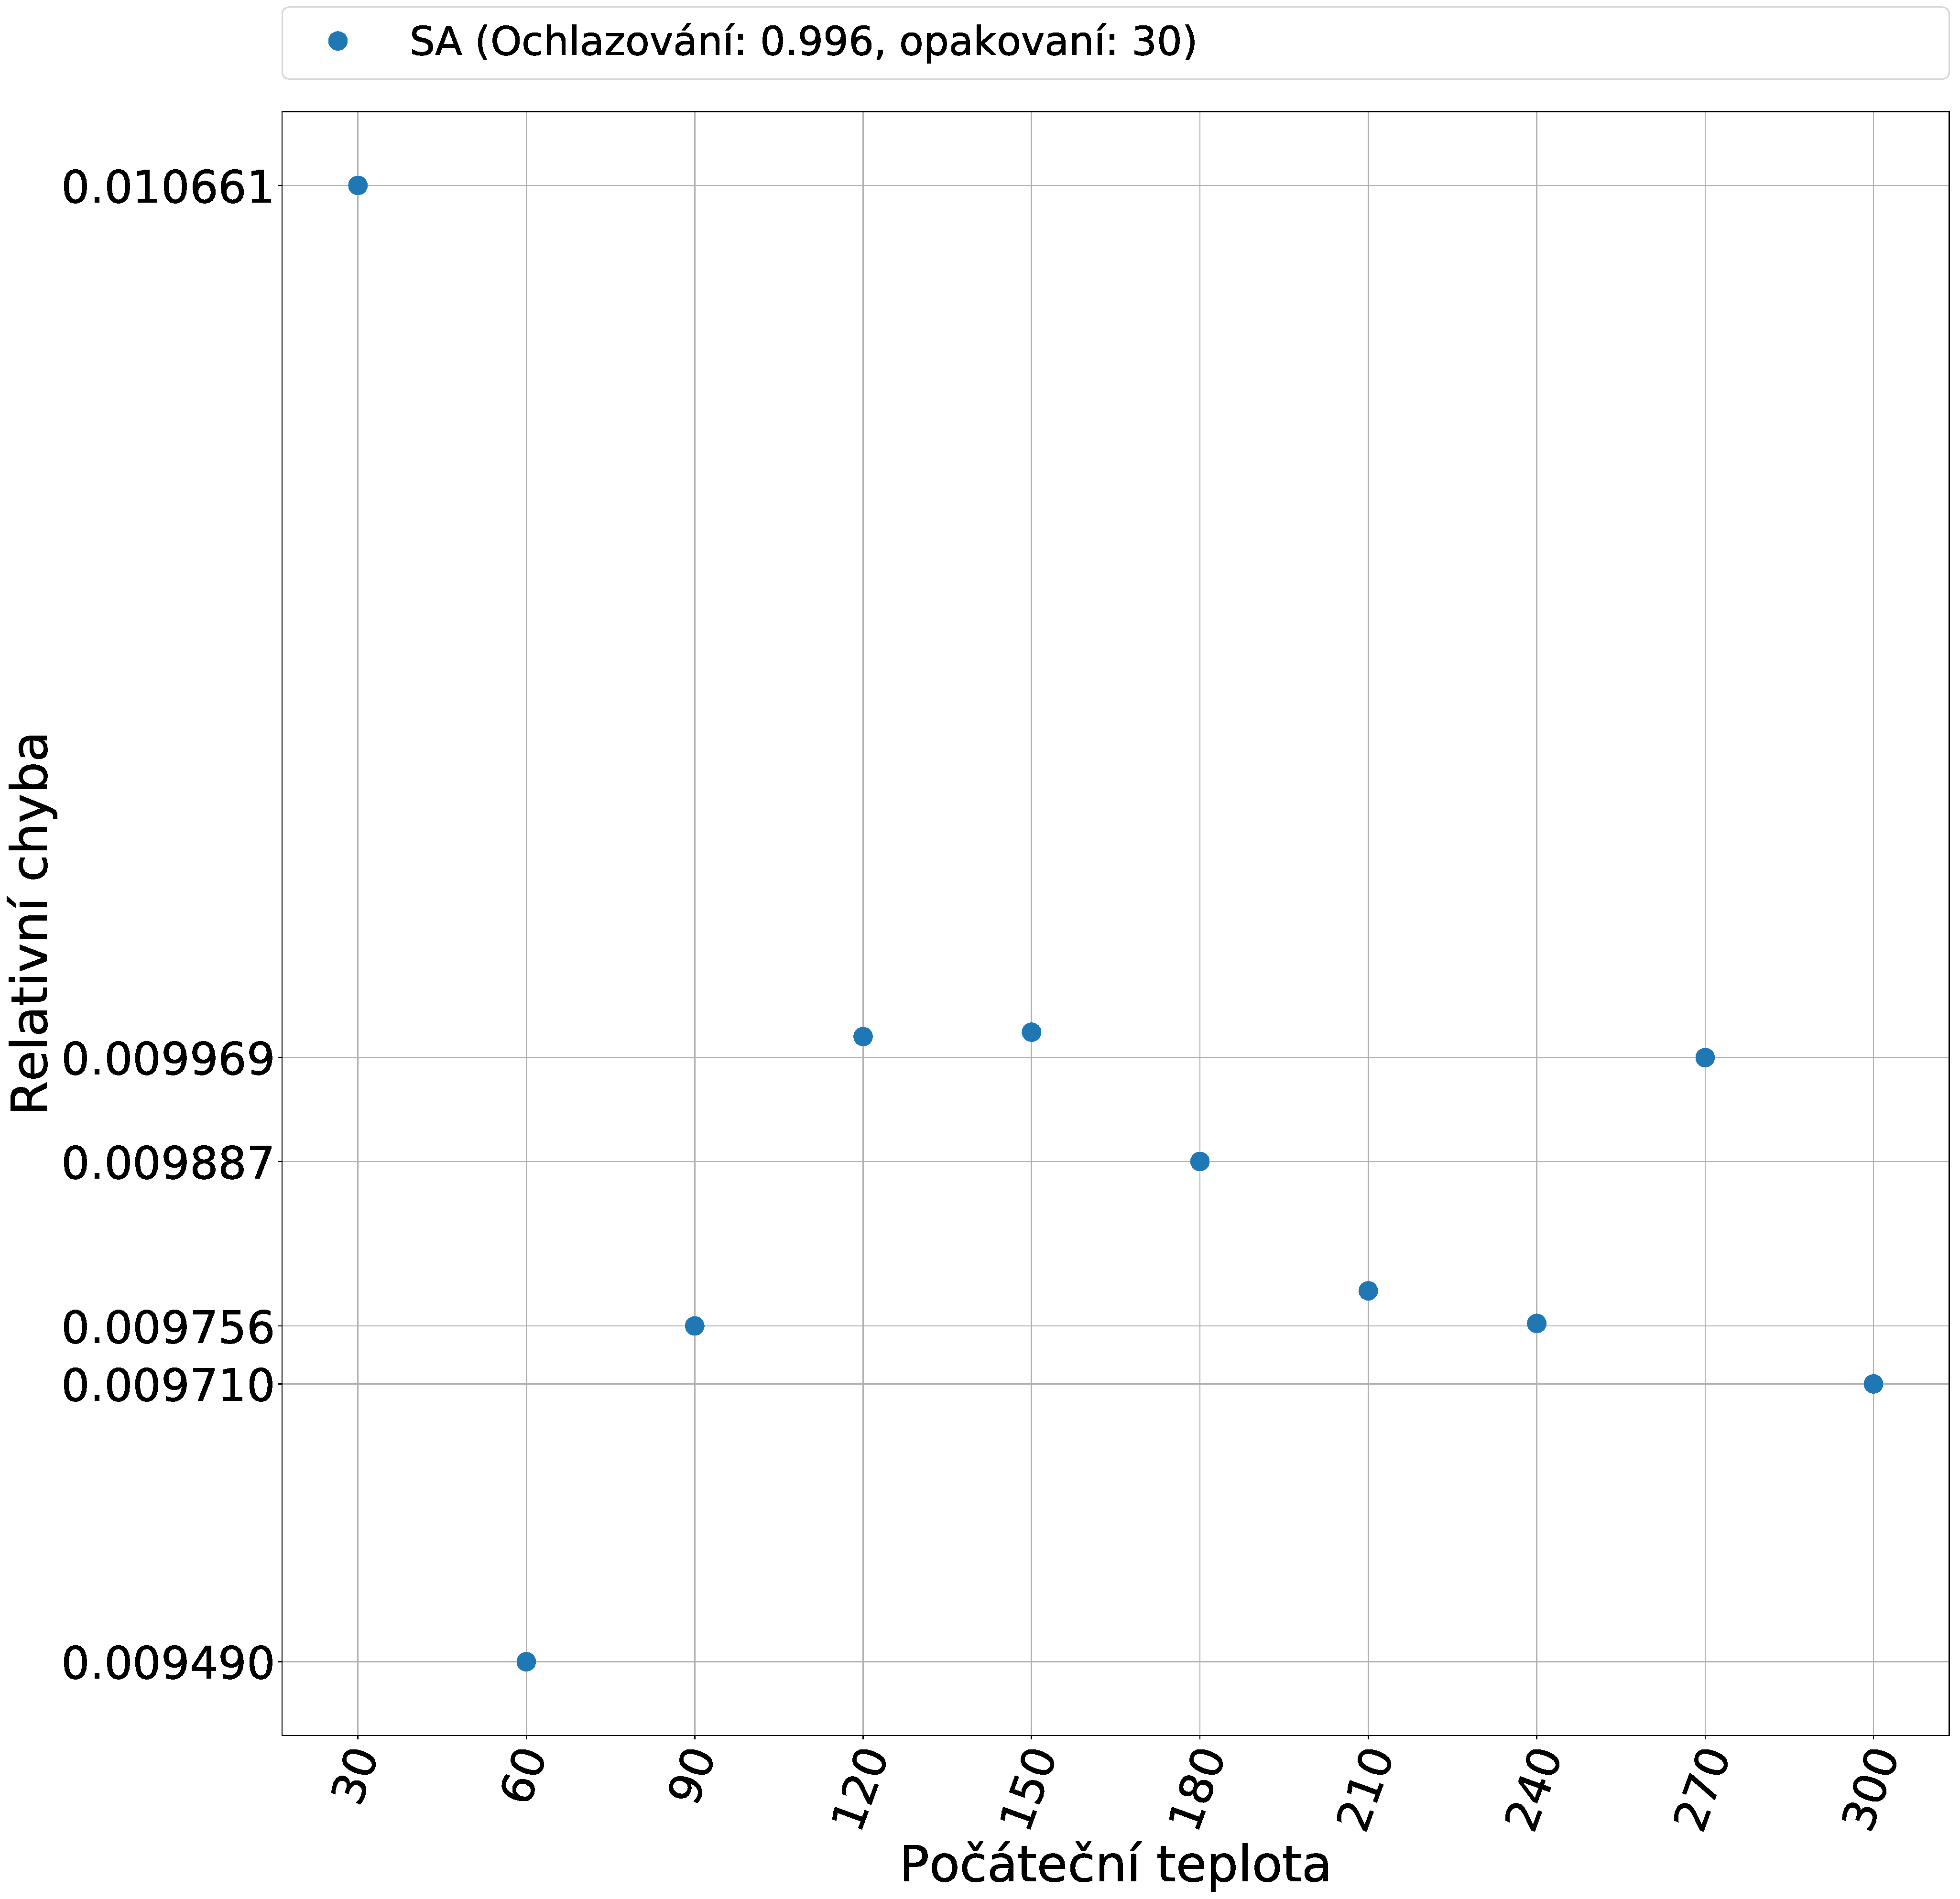
\includegraphics[width=\textwidth]{img/TE.pdf} 
    \end{minipage}
    \begin{minipage}[c]{0.49\textwidth}
        \centering 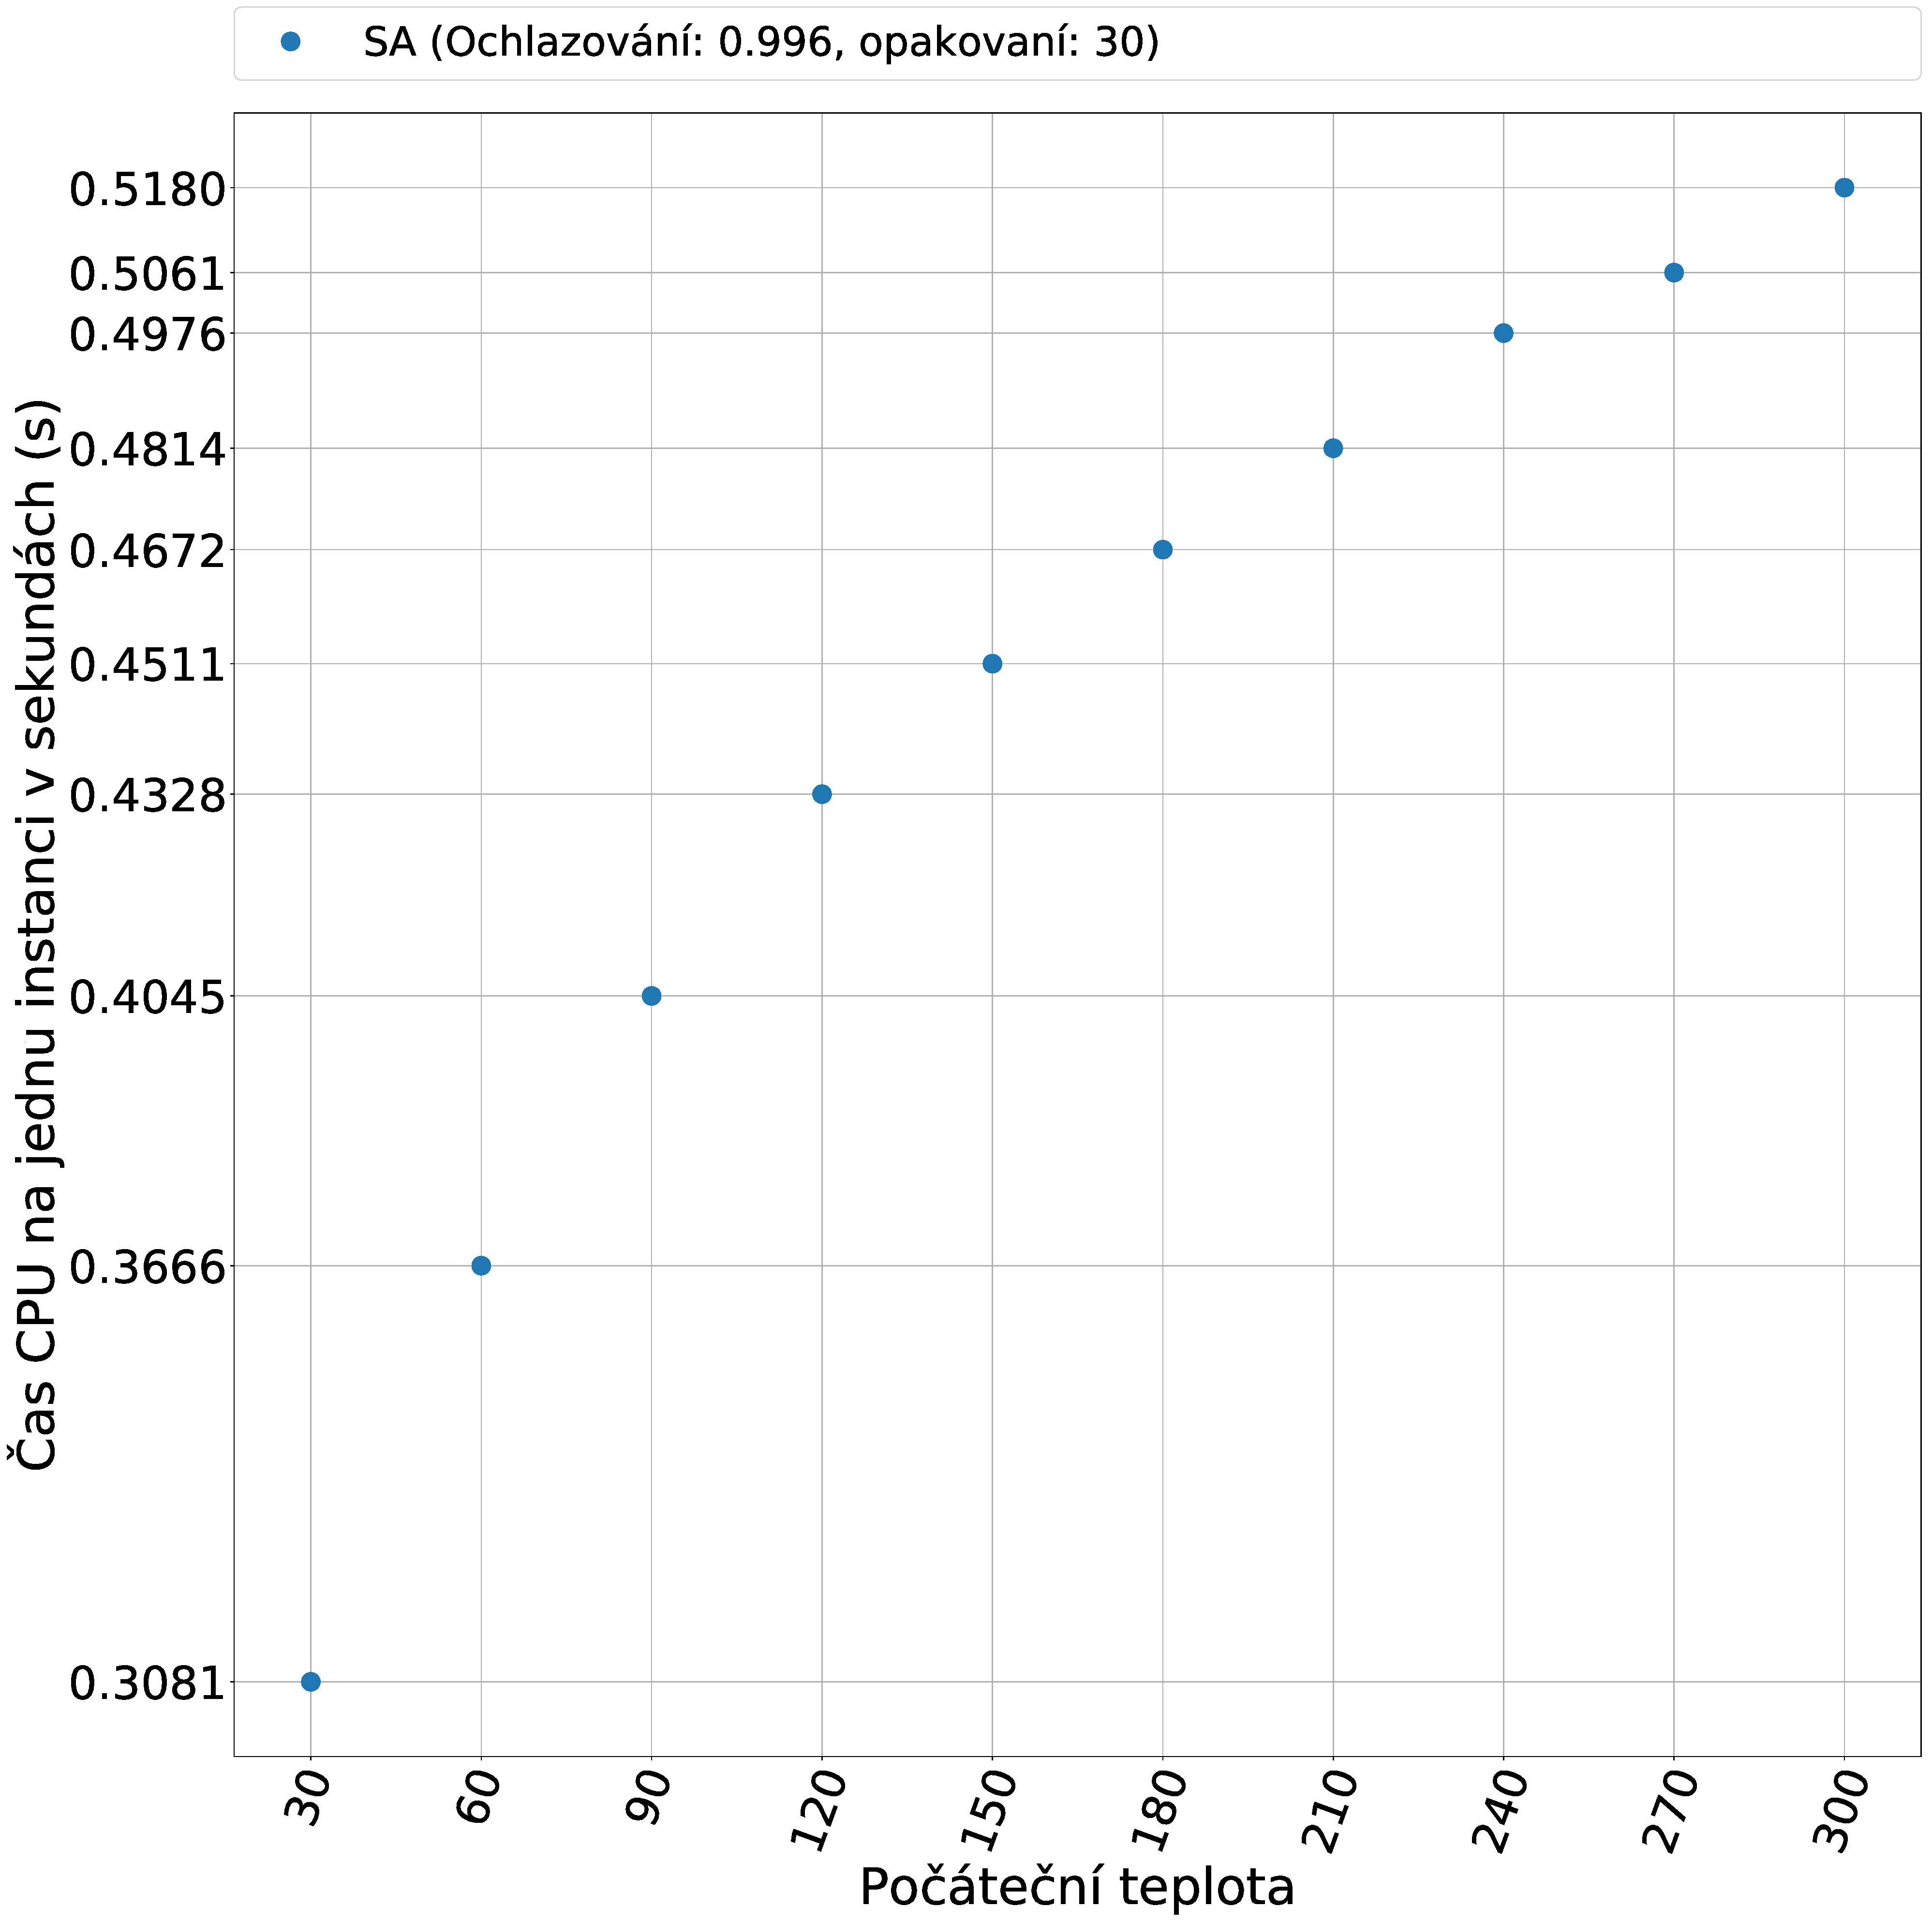
\includegraphics[width=\textwidth]{img/TT.pdf} 
    \end{minipage}
    \\
   \caption{Na levém grafu je závislost relativní chyby na počáteční teplotě. Na pravém grafu je závislost výpočetního času na počáteční teplotě}\label{fig:GVI}
\end{figure} 

\begin{figure}
	\centering
    \begin{minipage}[c]{0.325\textwidth}
        \centering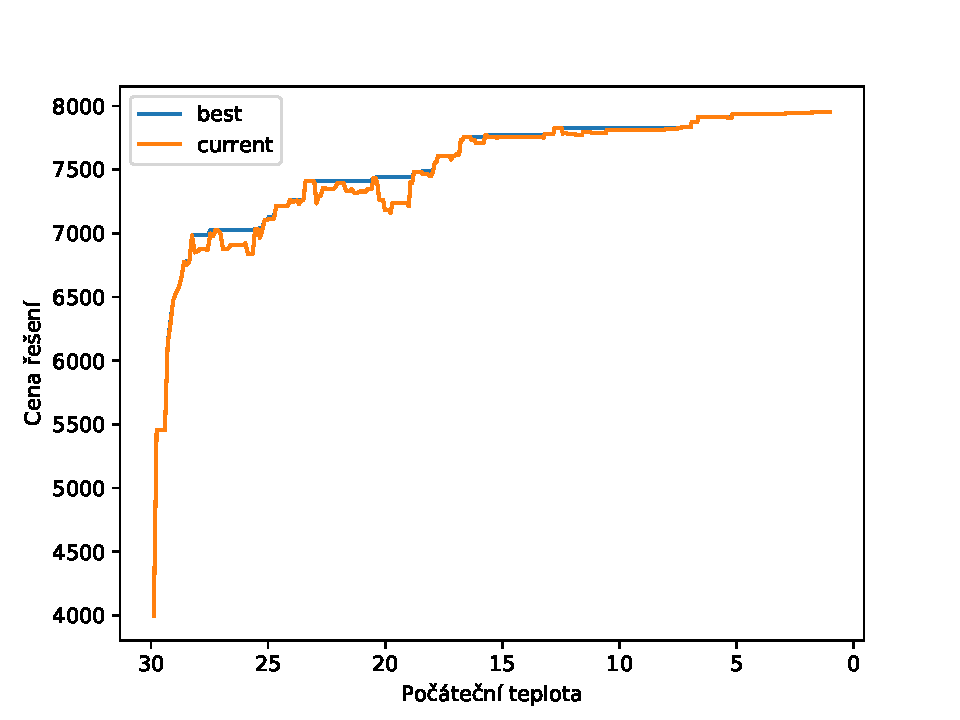
\includegraphics[width=\textwidth]{img/T30.pdf} 
    \end{minipage}
    \begin{minipage}[c]{0.325\textwidth}
        \centering 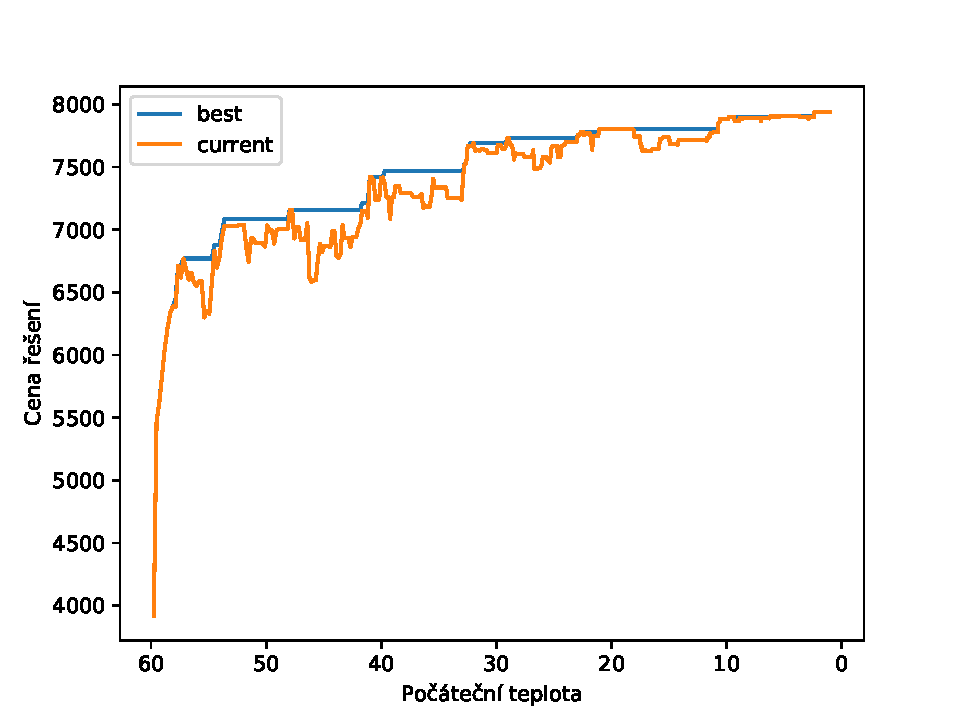
\includegraphics[width=\textwidth]{img/T60.pdf} 
    \end{minipage}
    \begin{minipage}[c]{0.325\textwidth}
        \centering 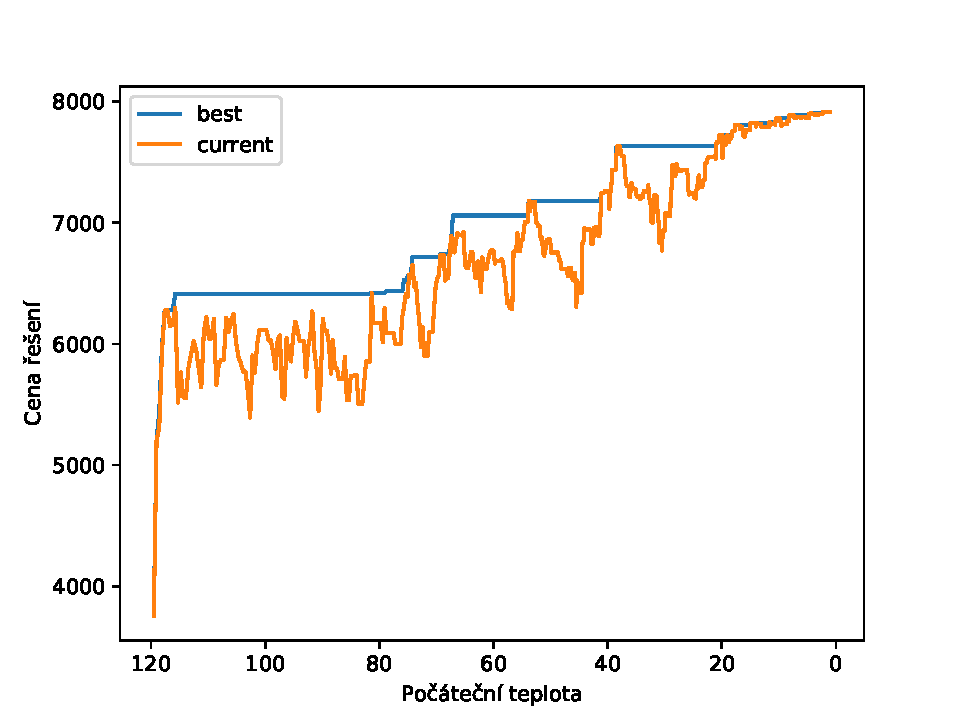
\includegraphics[width=\textwidth]{img/T120.pdf} 
    \end{minipage}
    \\
    \begin{minipage}[c]{0.49\textwidth}
        \centering 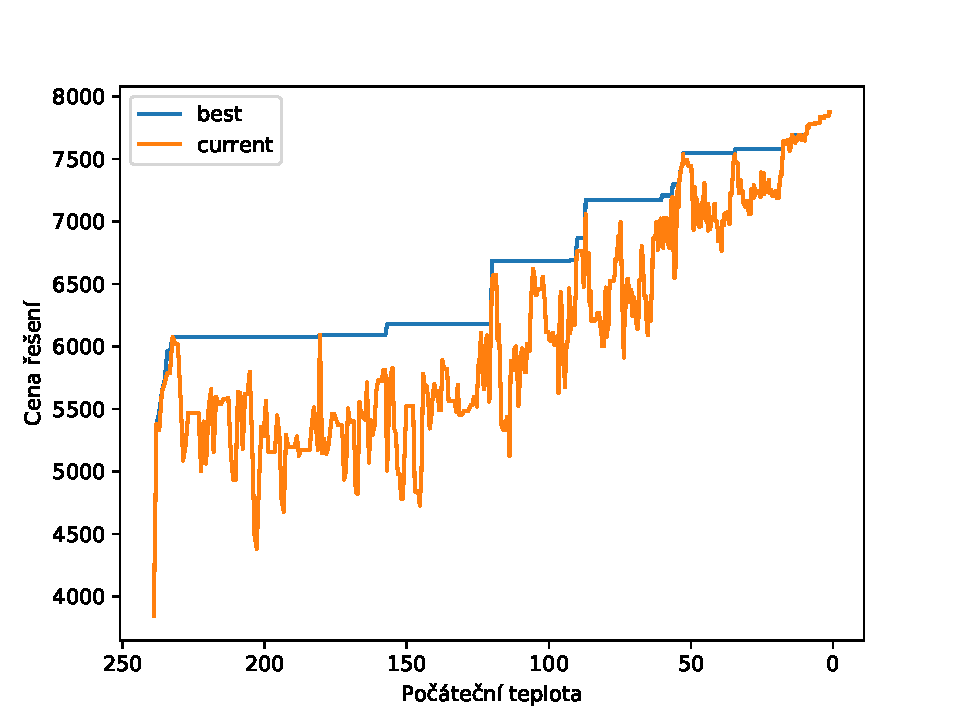
\includegraphics[width=\textwidth]{img/T240.pdf} 
    \end{minipage}
    \begin{minipage}[c]{0.49\textwidth}
        \centering 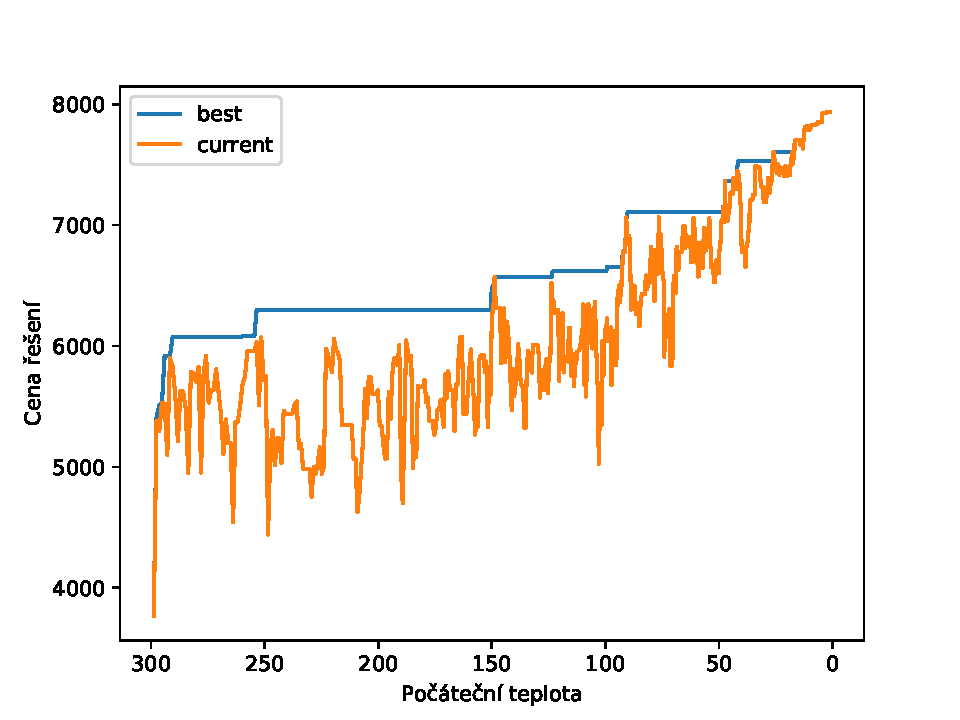
\includegraphics[width=\textwidth]{img/T300.pdf} 
    \end{minipage}
   \caption{Na levém grafu je závislost relativní chyby na počáteční teplotě. Na pravém grafu je závislost výpočetního času na počáteční teplotě}\label{fig:GVI}
\end{figure} 



\subsection{Závislost na koeficientu ochlazování}
\begin{figure}
	\centering
    \begin{minipage}[c]{0.49\textwidth}
        \centering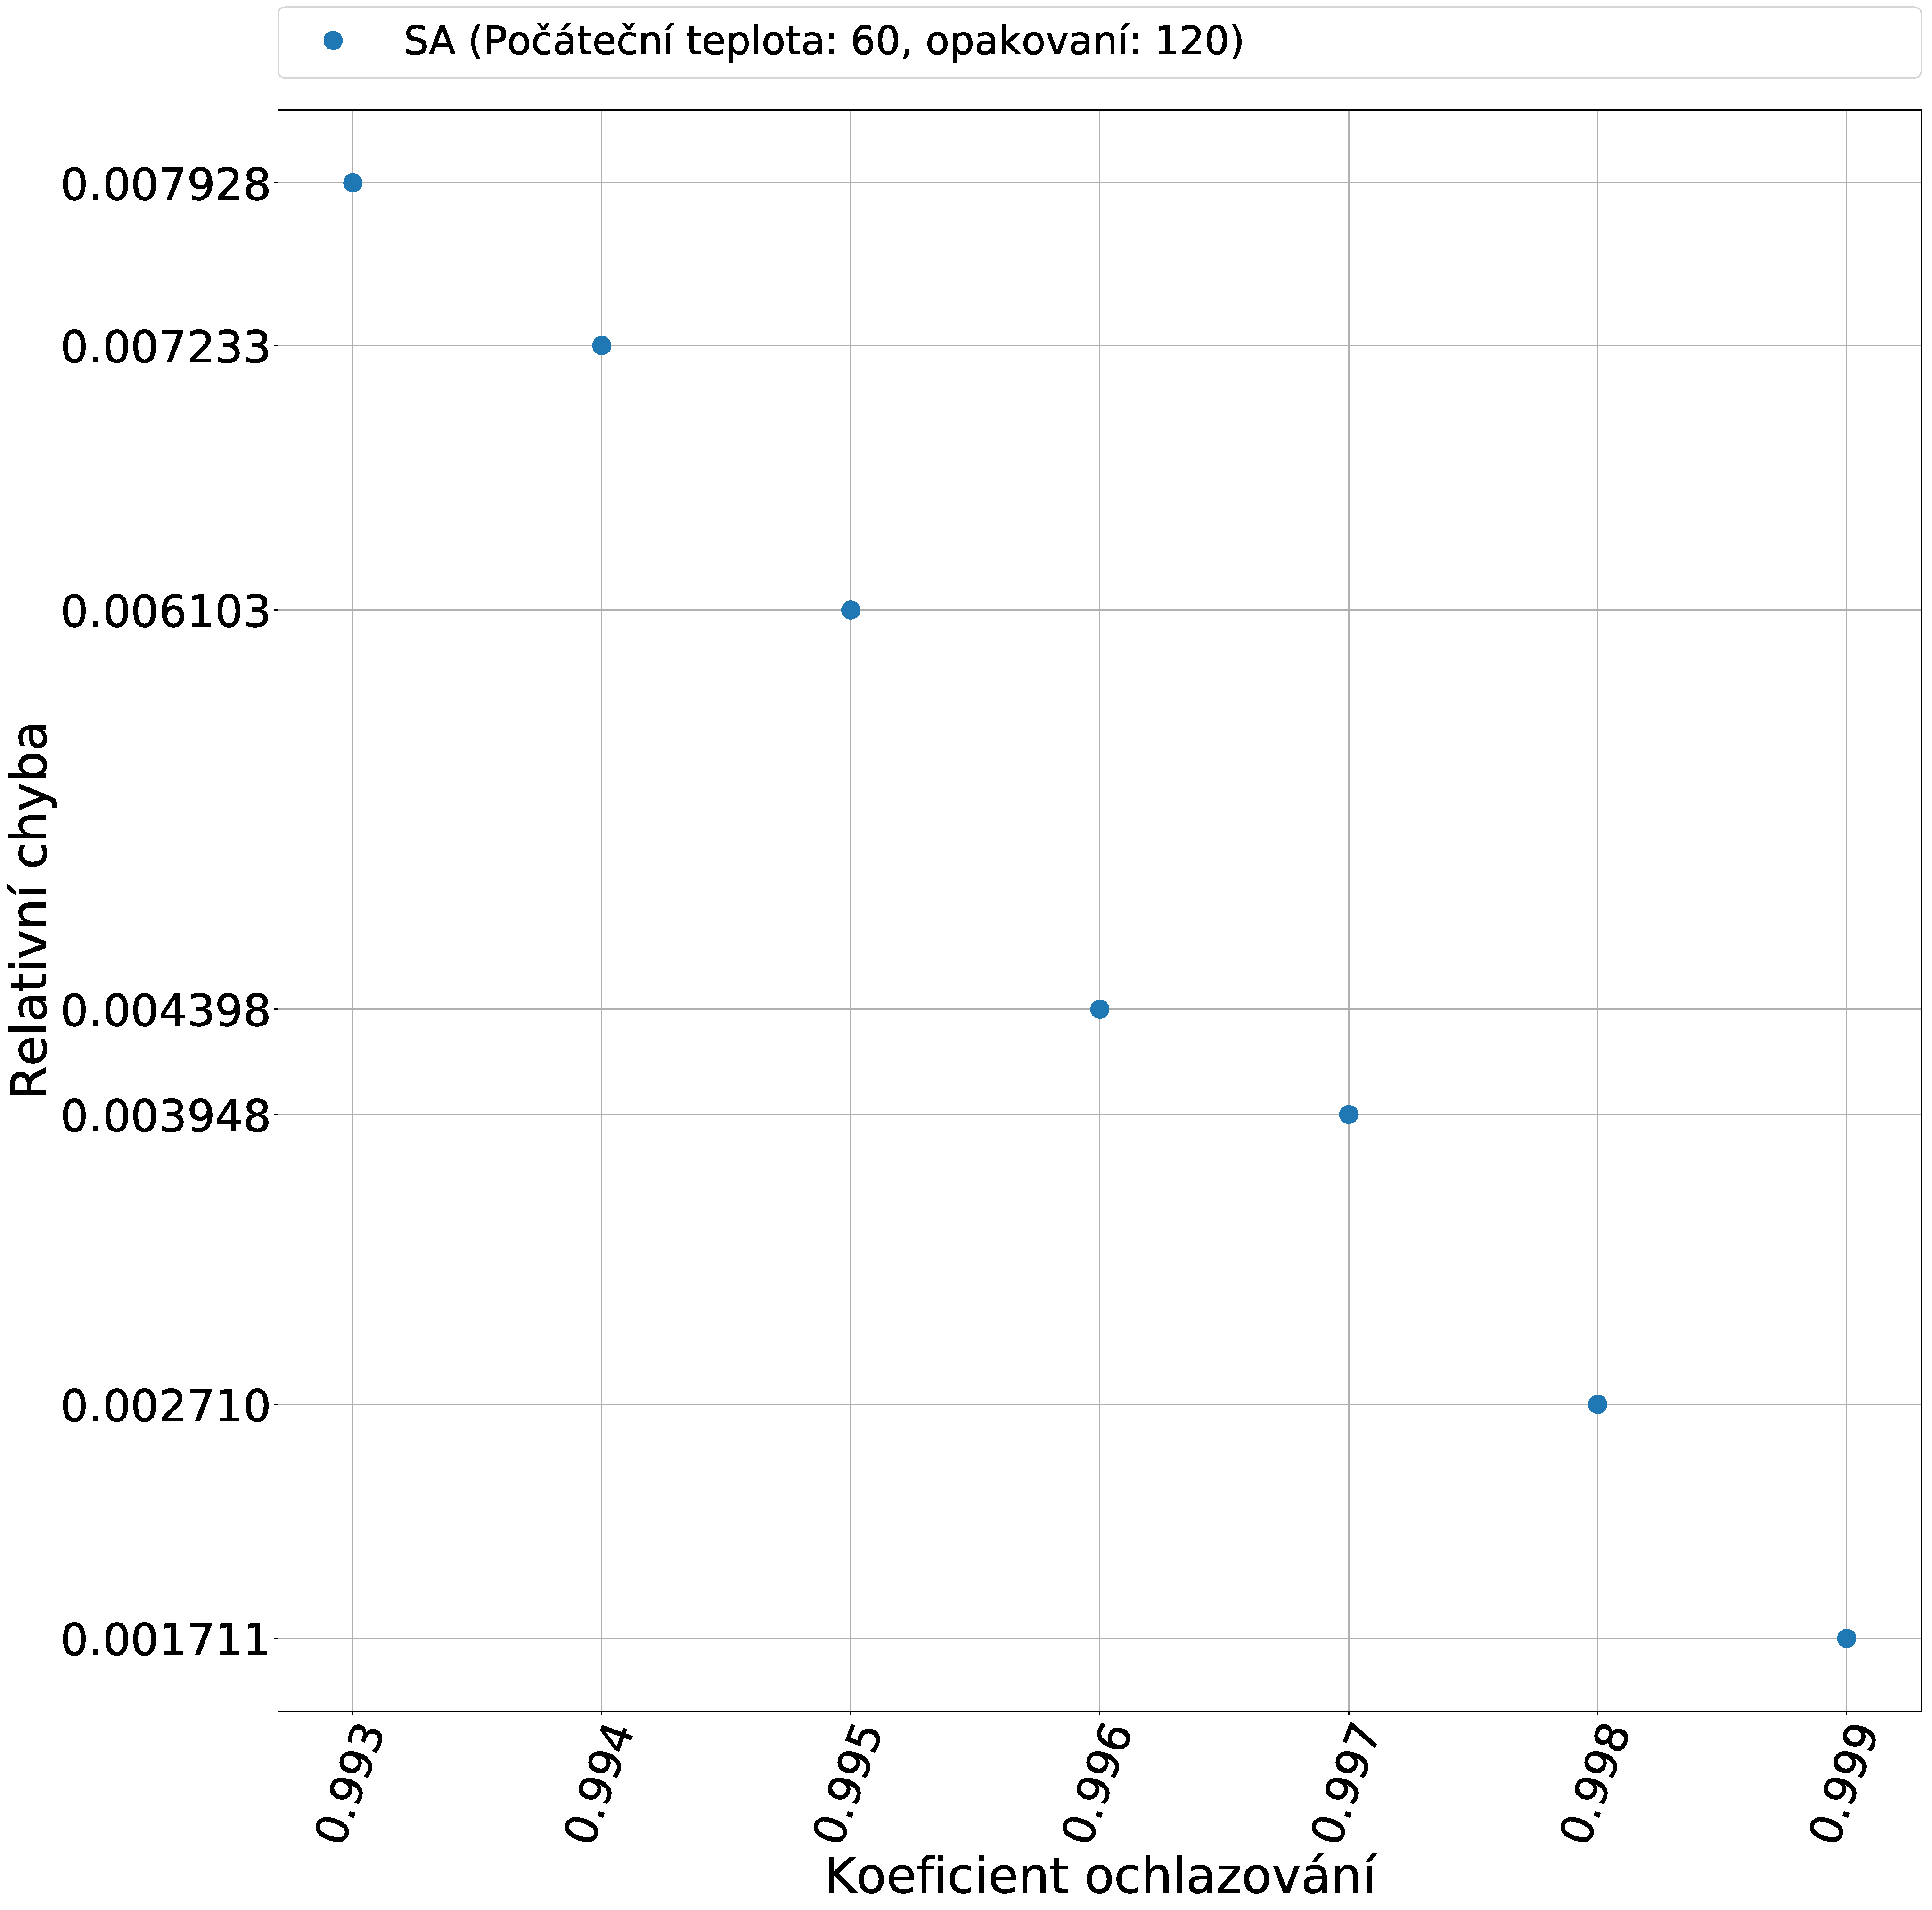
\includegraphics[width=\textwidth]{img/KE.pdf} 
    \end{minipage}
    \begin{minipage}[c]{0.49\textwidth}
        \centering 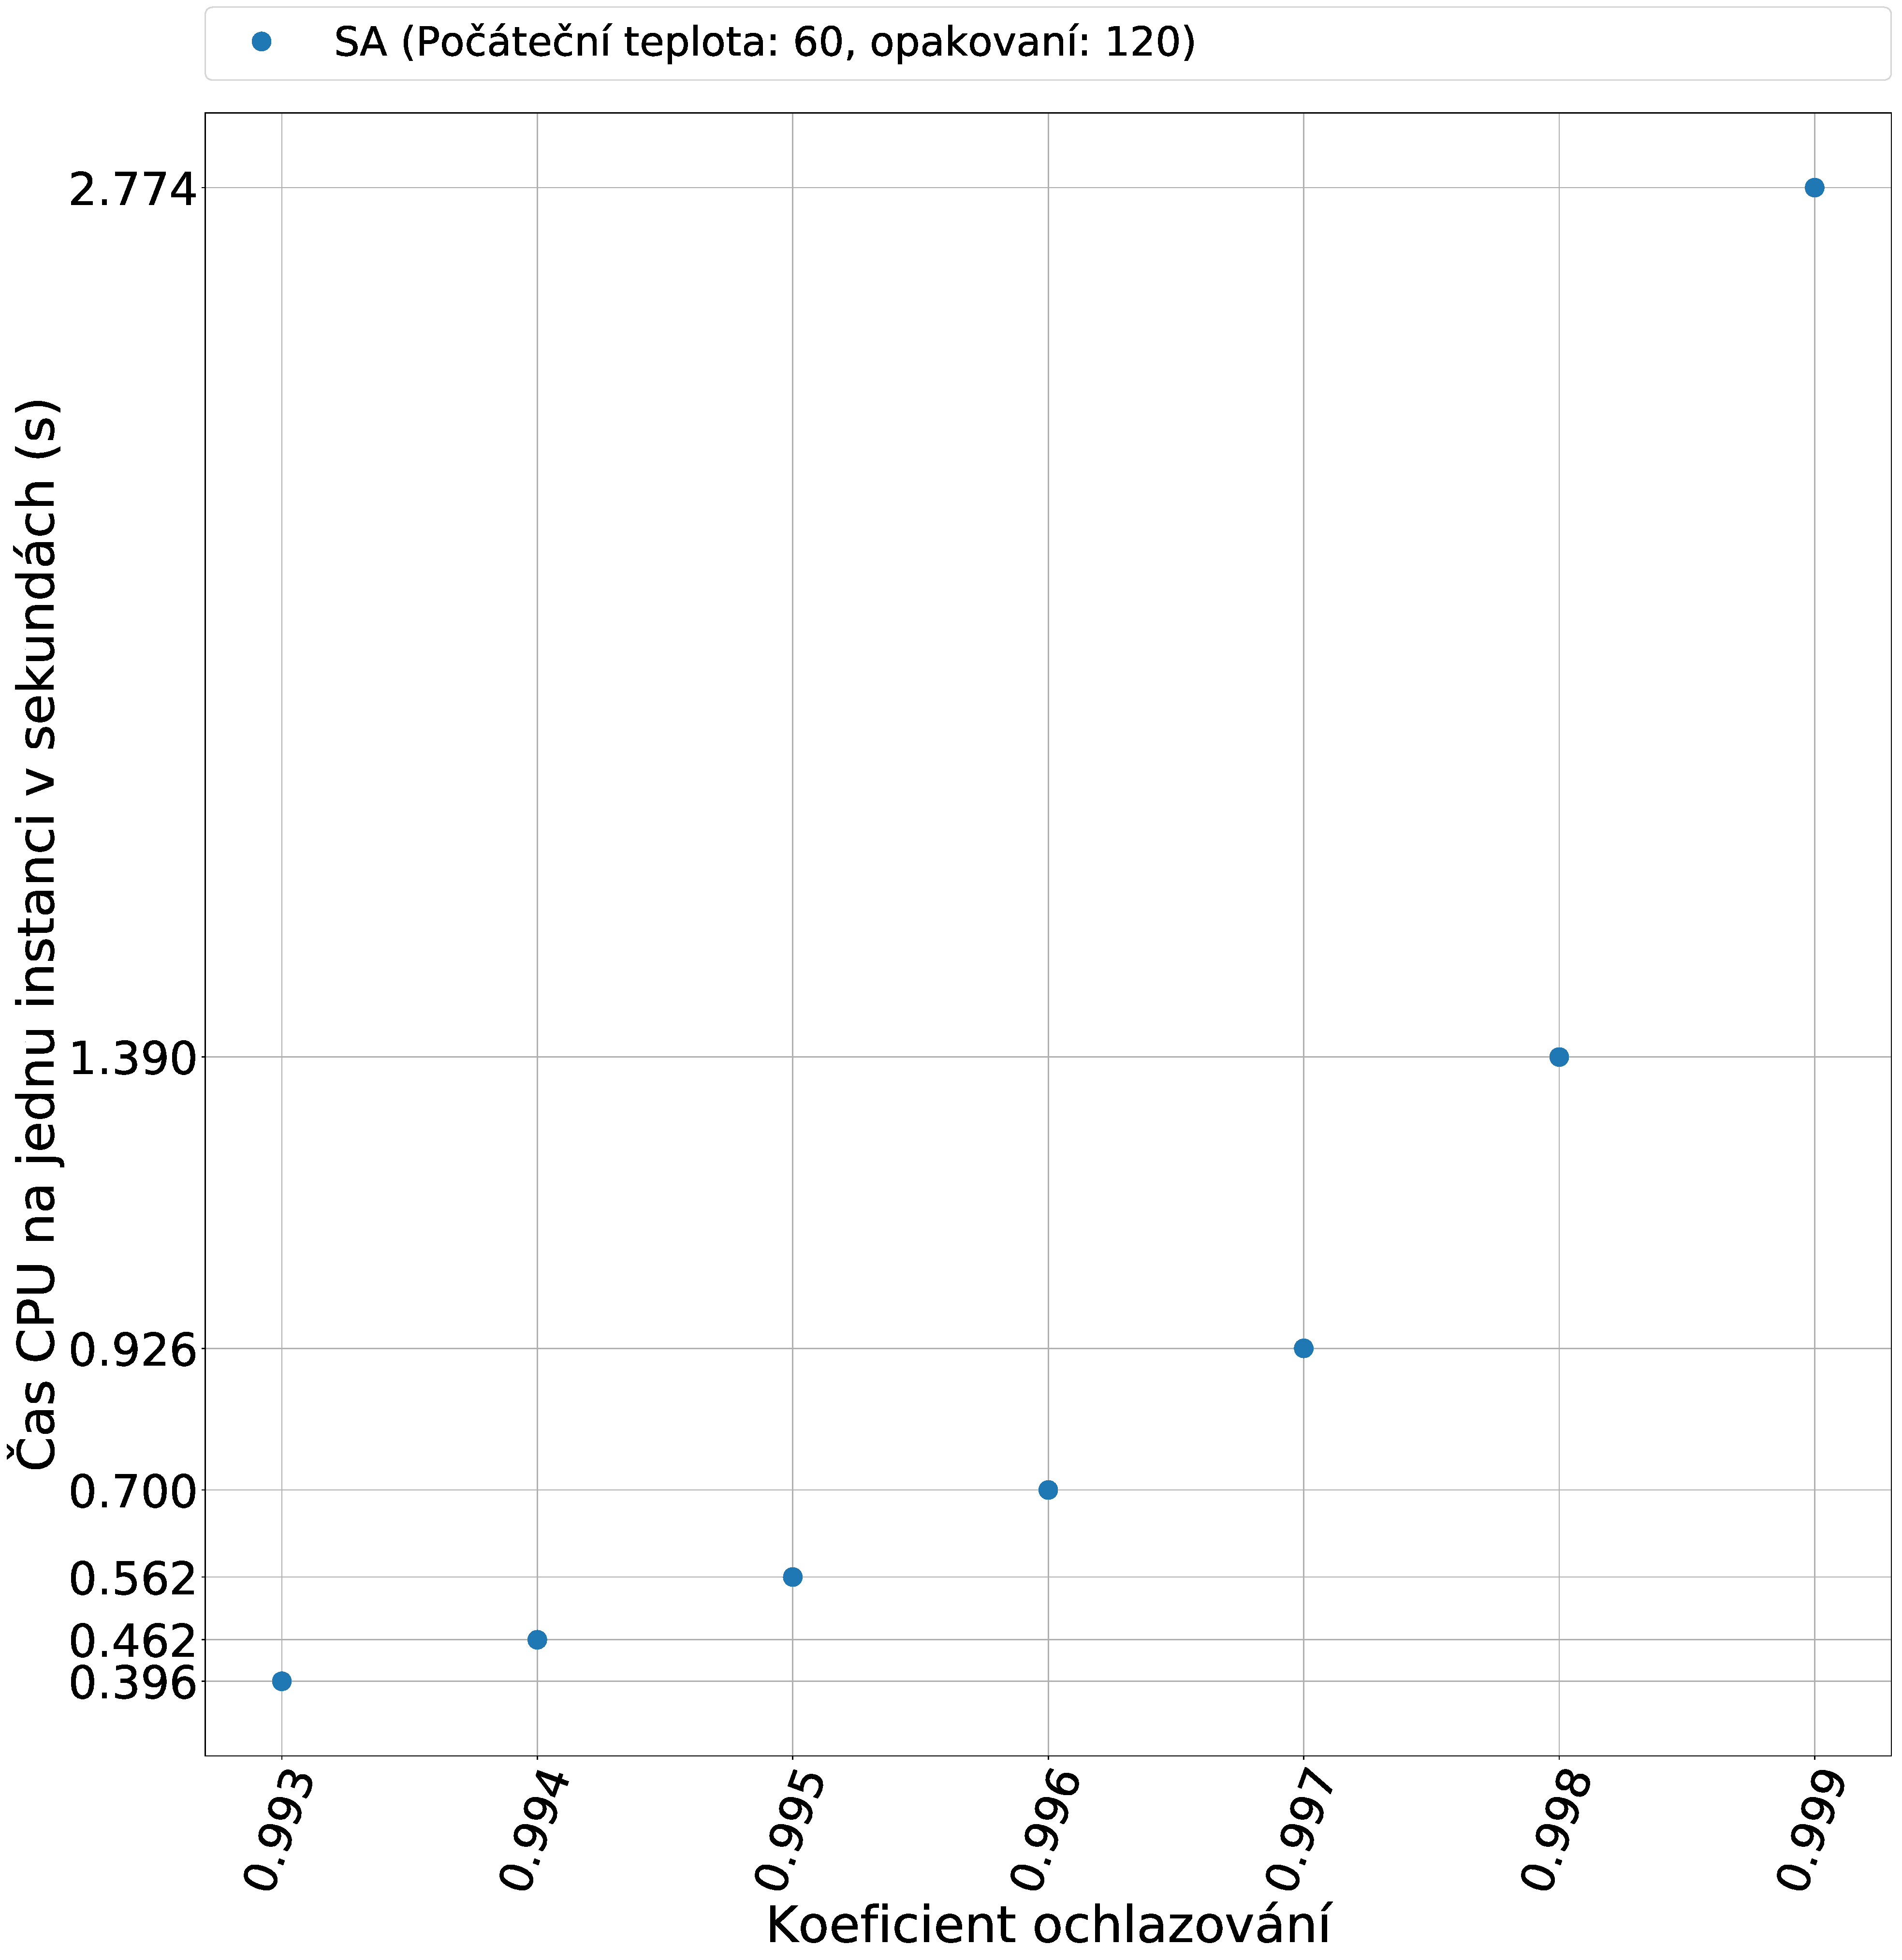
\includegraphics[width=\textwidth]{img/KT.pdf} 
    \end{minipage}
    \\
   \caption{Na levém grafu je závislost relativní chyby na koeficientu ochlazování. Na pravém grafu je závislost výpočetního času na koeficientu ochlazování}\label{fig:GVI}
\end{figure} 

\begin{figure}
	\centering
    \begin{minipage}[c]{0.49\textwidth}
        \centering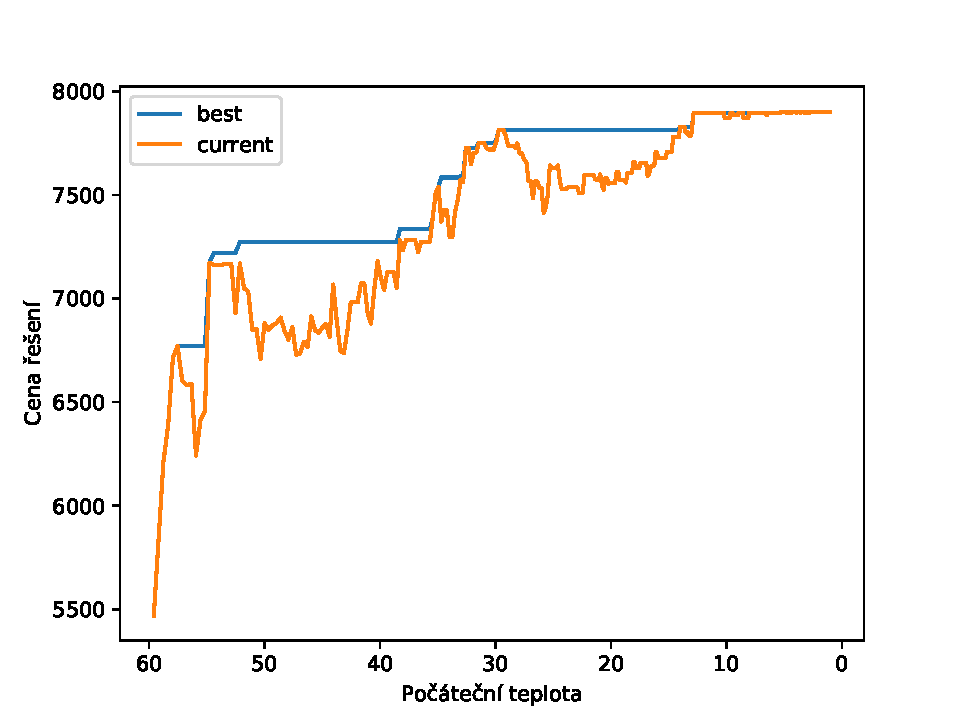
\includegraphics[width=\textwidth]{img/993.pdf} 
    \end{minipage}
    \begin{minipage}[c]{0.48\textwidth}
        \centering 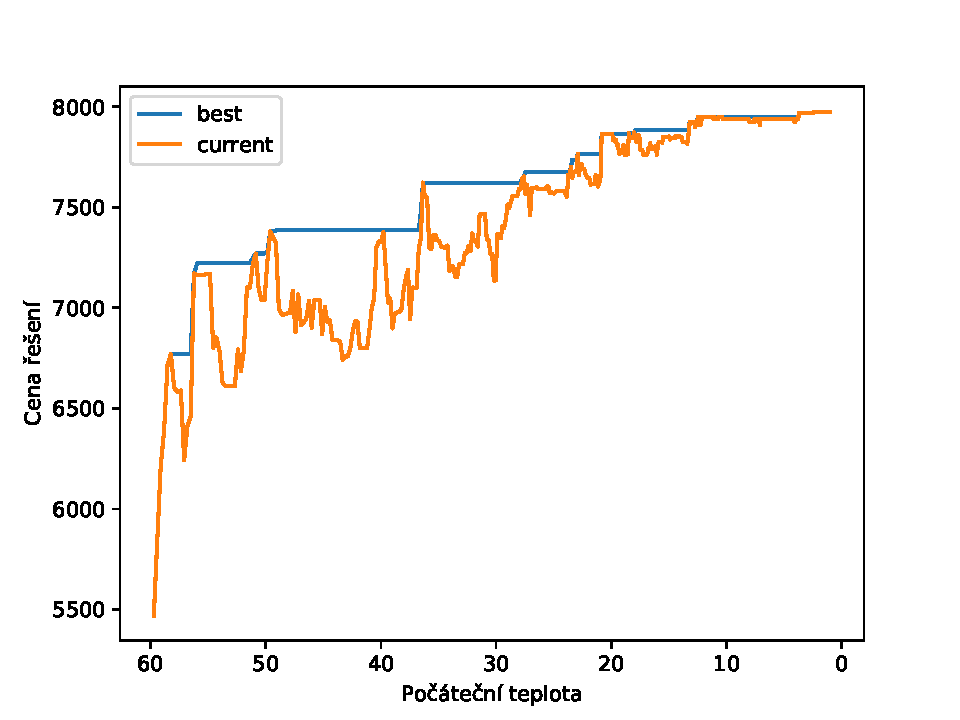
\includegraphics[width=\textwidth]{img/995.pdf} 
    \end{minipage}
    \\
    \begin{minipage}[c]{0.49\textwidth}
        \centering 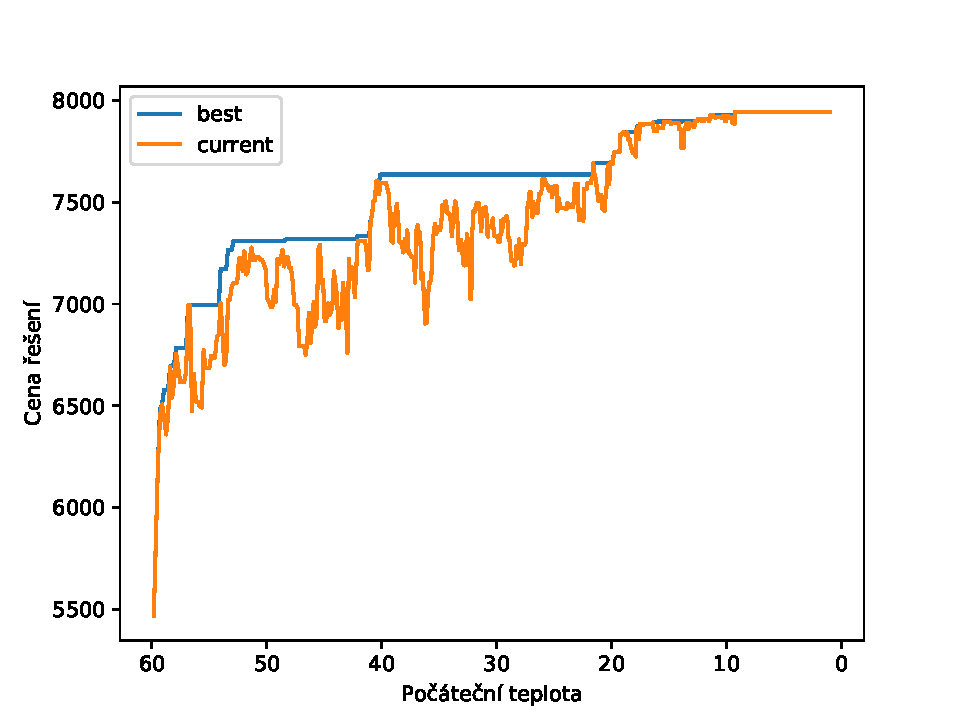
\includegraphics[width=\textwidth]{img/997.pdf} 
    \end{minipage}
    \begin{minipage}[c]{0.49\textwidth}
        \centering 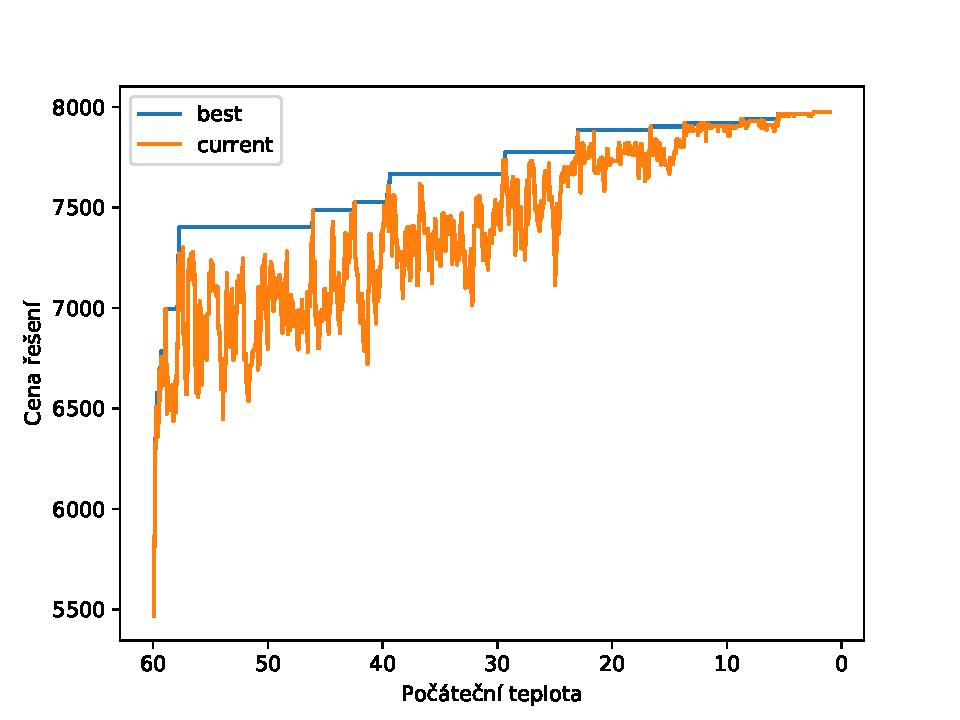
\includegraphics[width=\textwidth]{img/999.pdf} 
    \end{minipage}
   \caption{Na levém grafu je závislost relativní chyby na počáteční teplotě. Na pravém grafu je závislost výpočetního času na počáteční teplotě}\label{fig:GVI}
\end{figure} 


\subsection{Závislost na počtu iterací na jedné teplotě}
 \begin{figure}
	\centering
    \begin{minipage}[c]{0.49\textwidth}
        \centering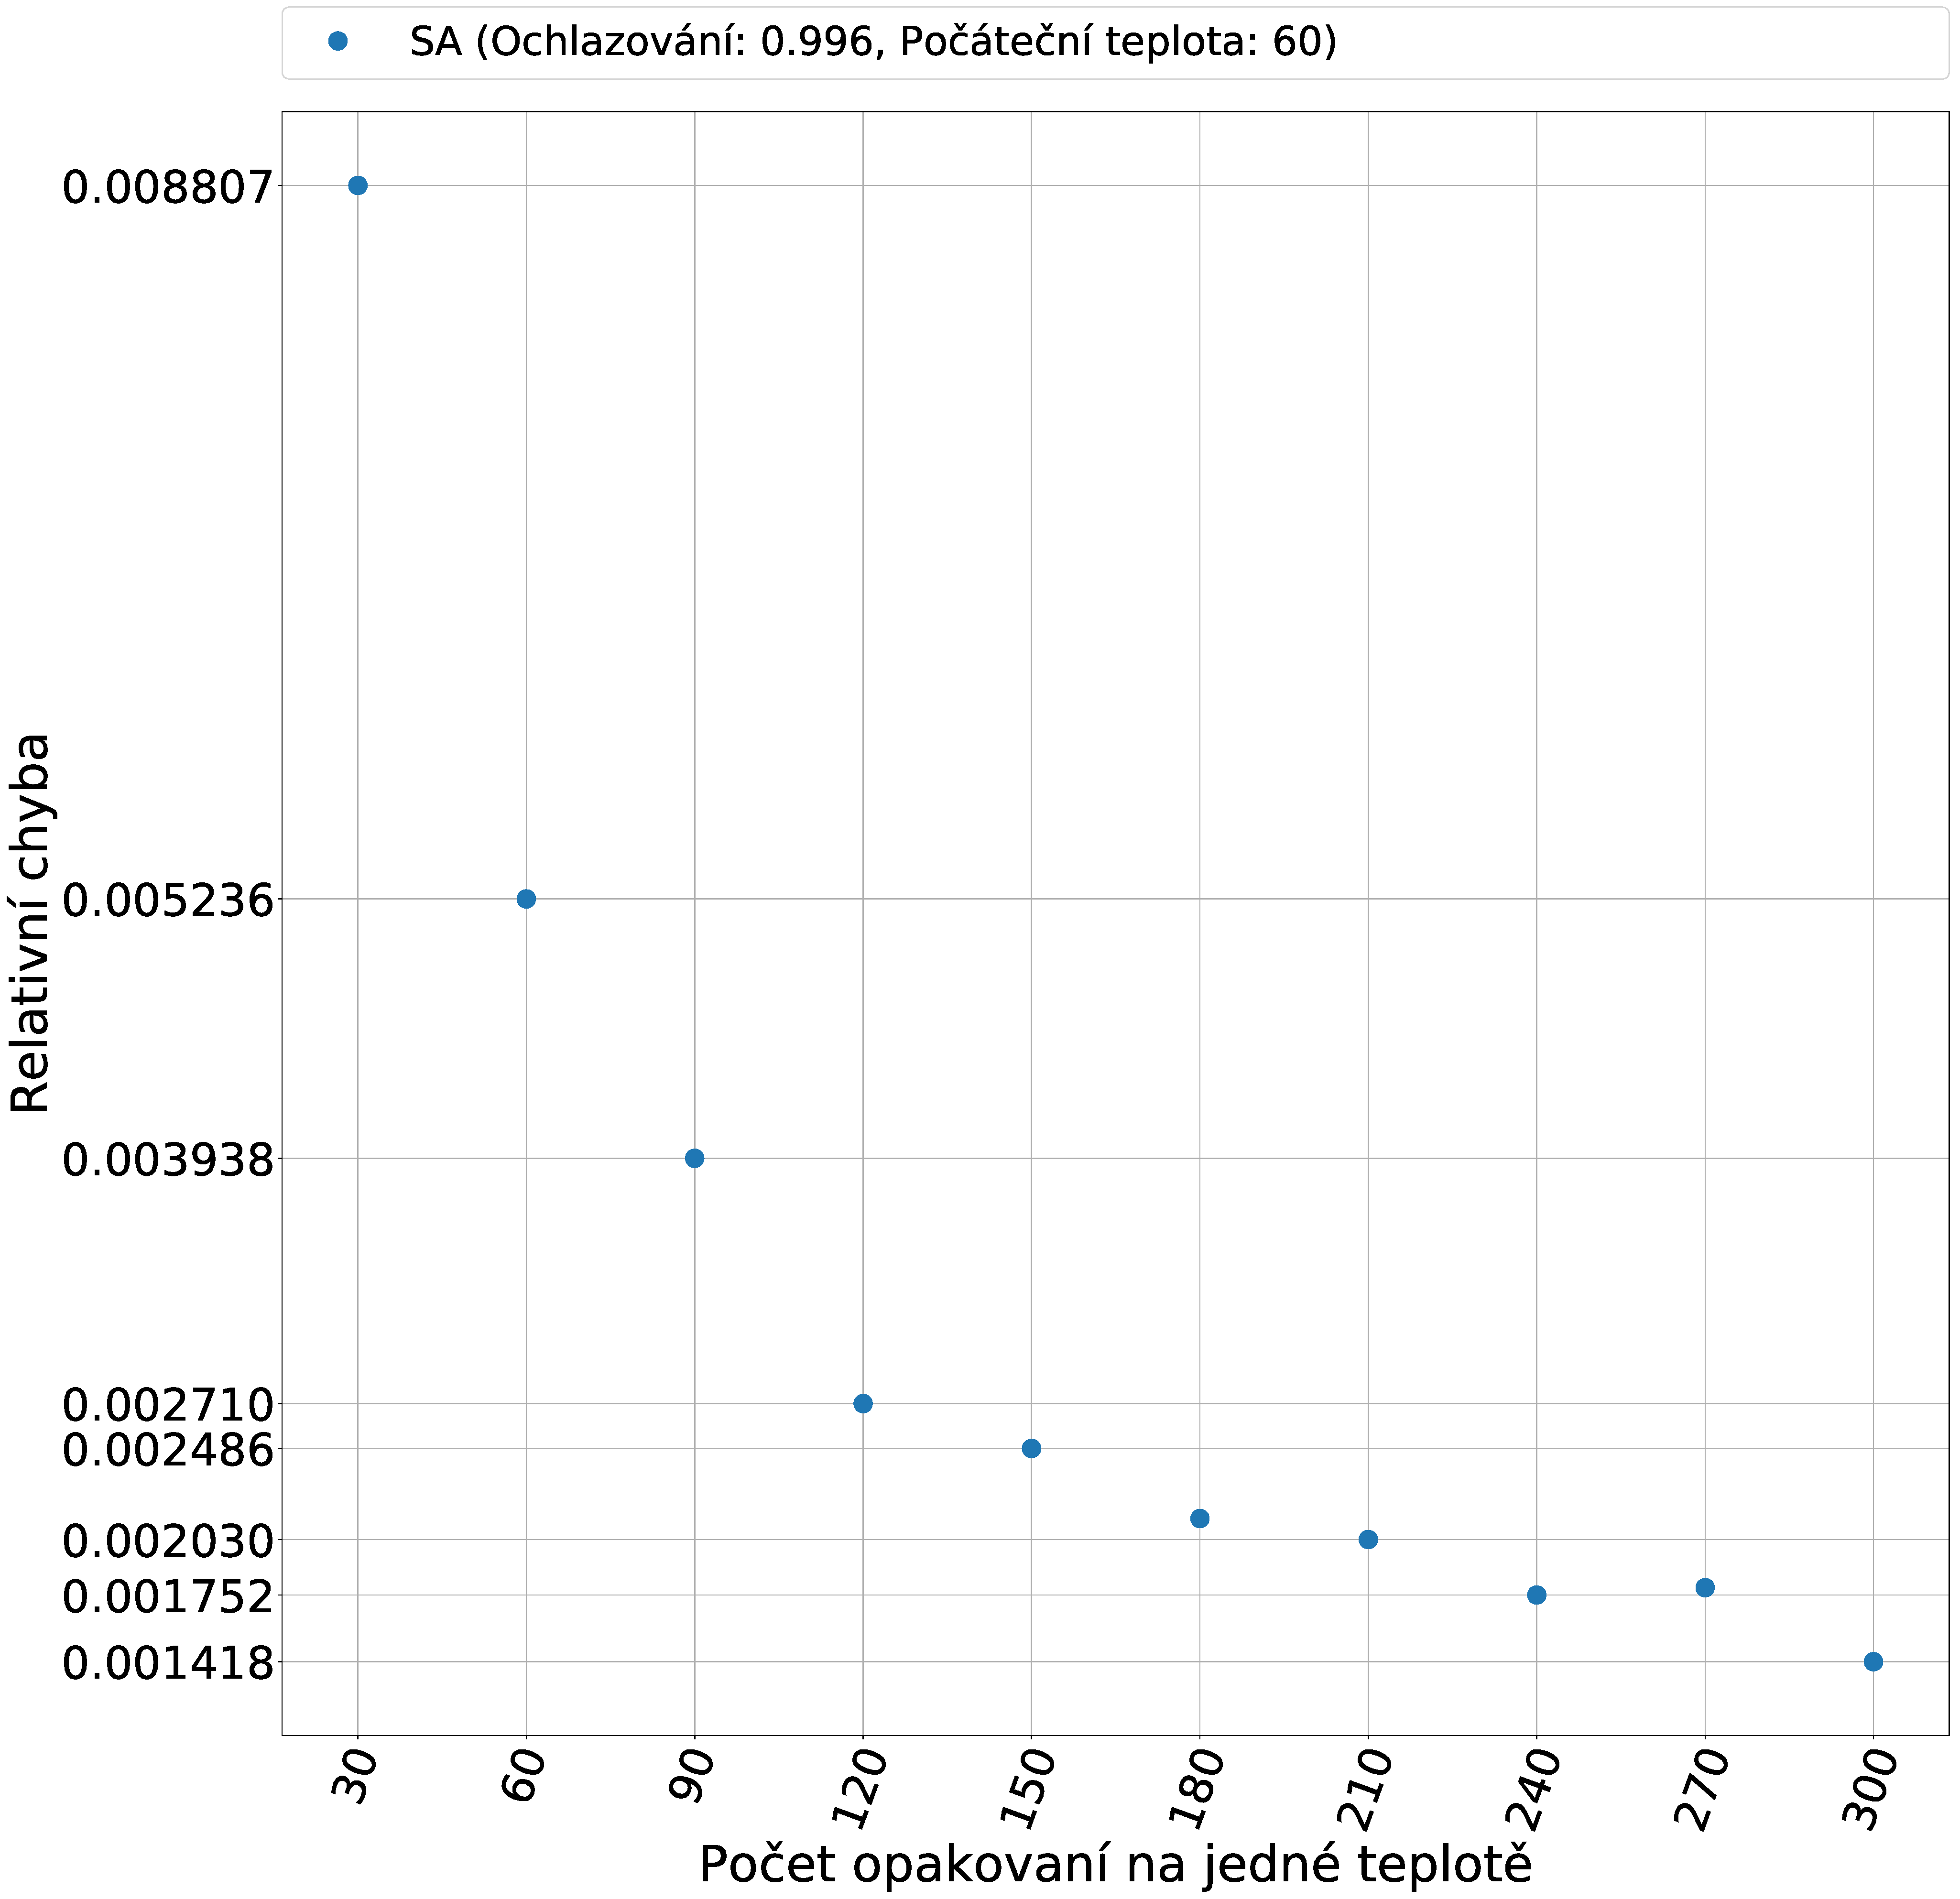
\includegraphics[width=\textwidth]{img/CE.pdf} 
    \end{minipage}
    \begin{minipage}[c]{0.49\textwidth}
        \centering 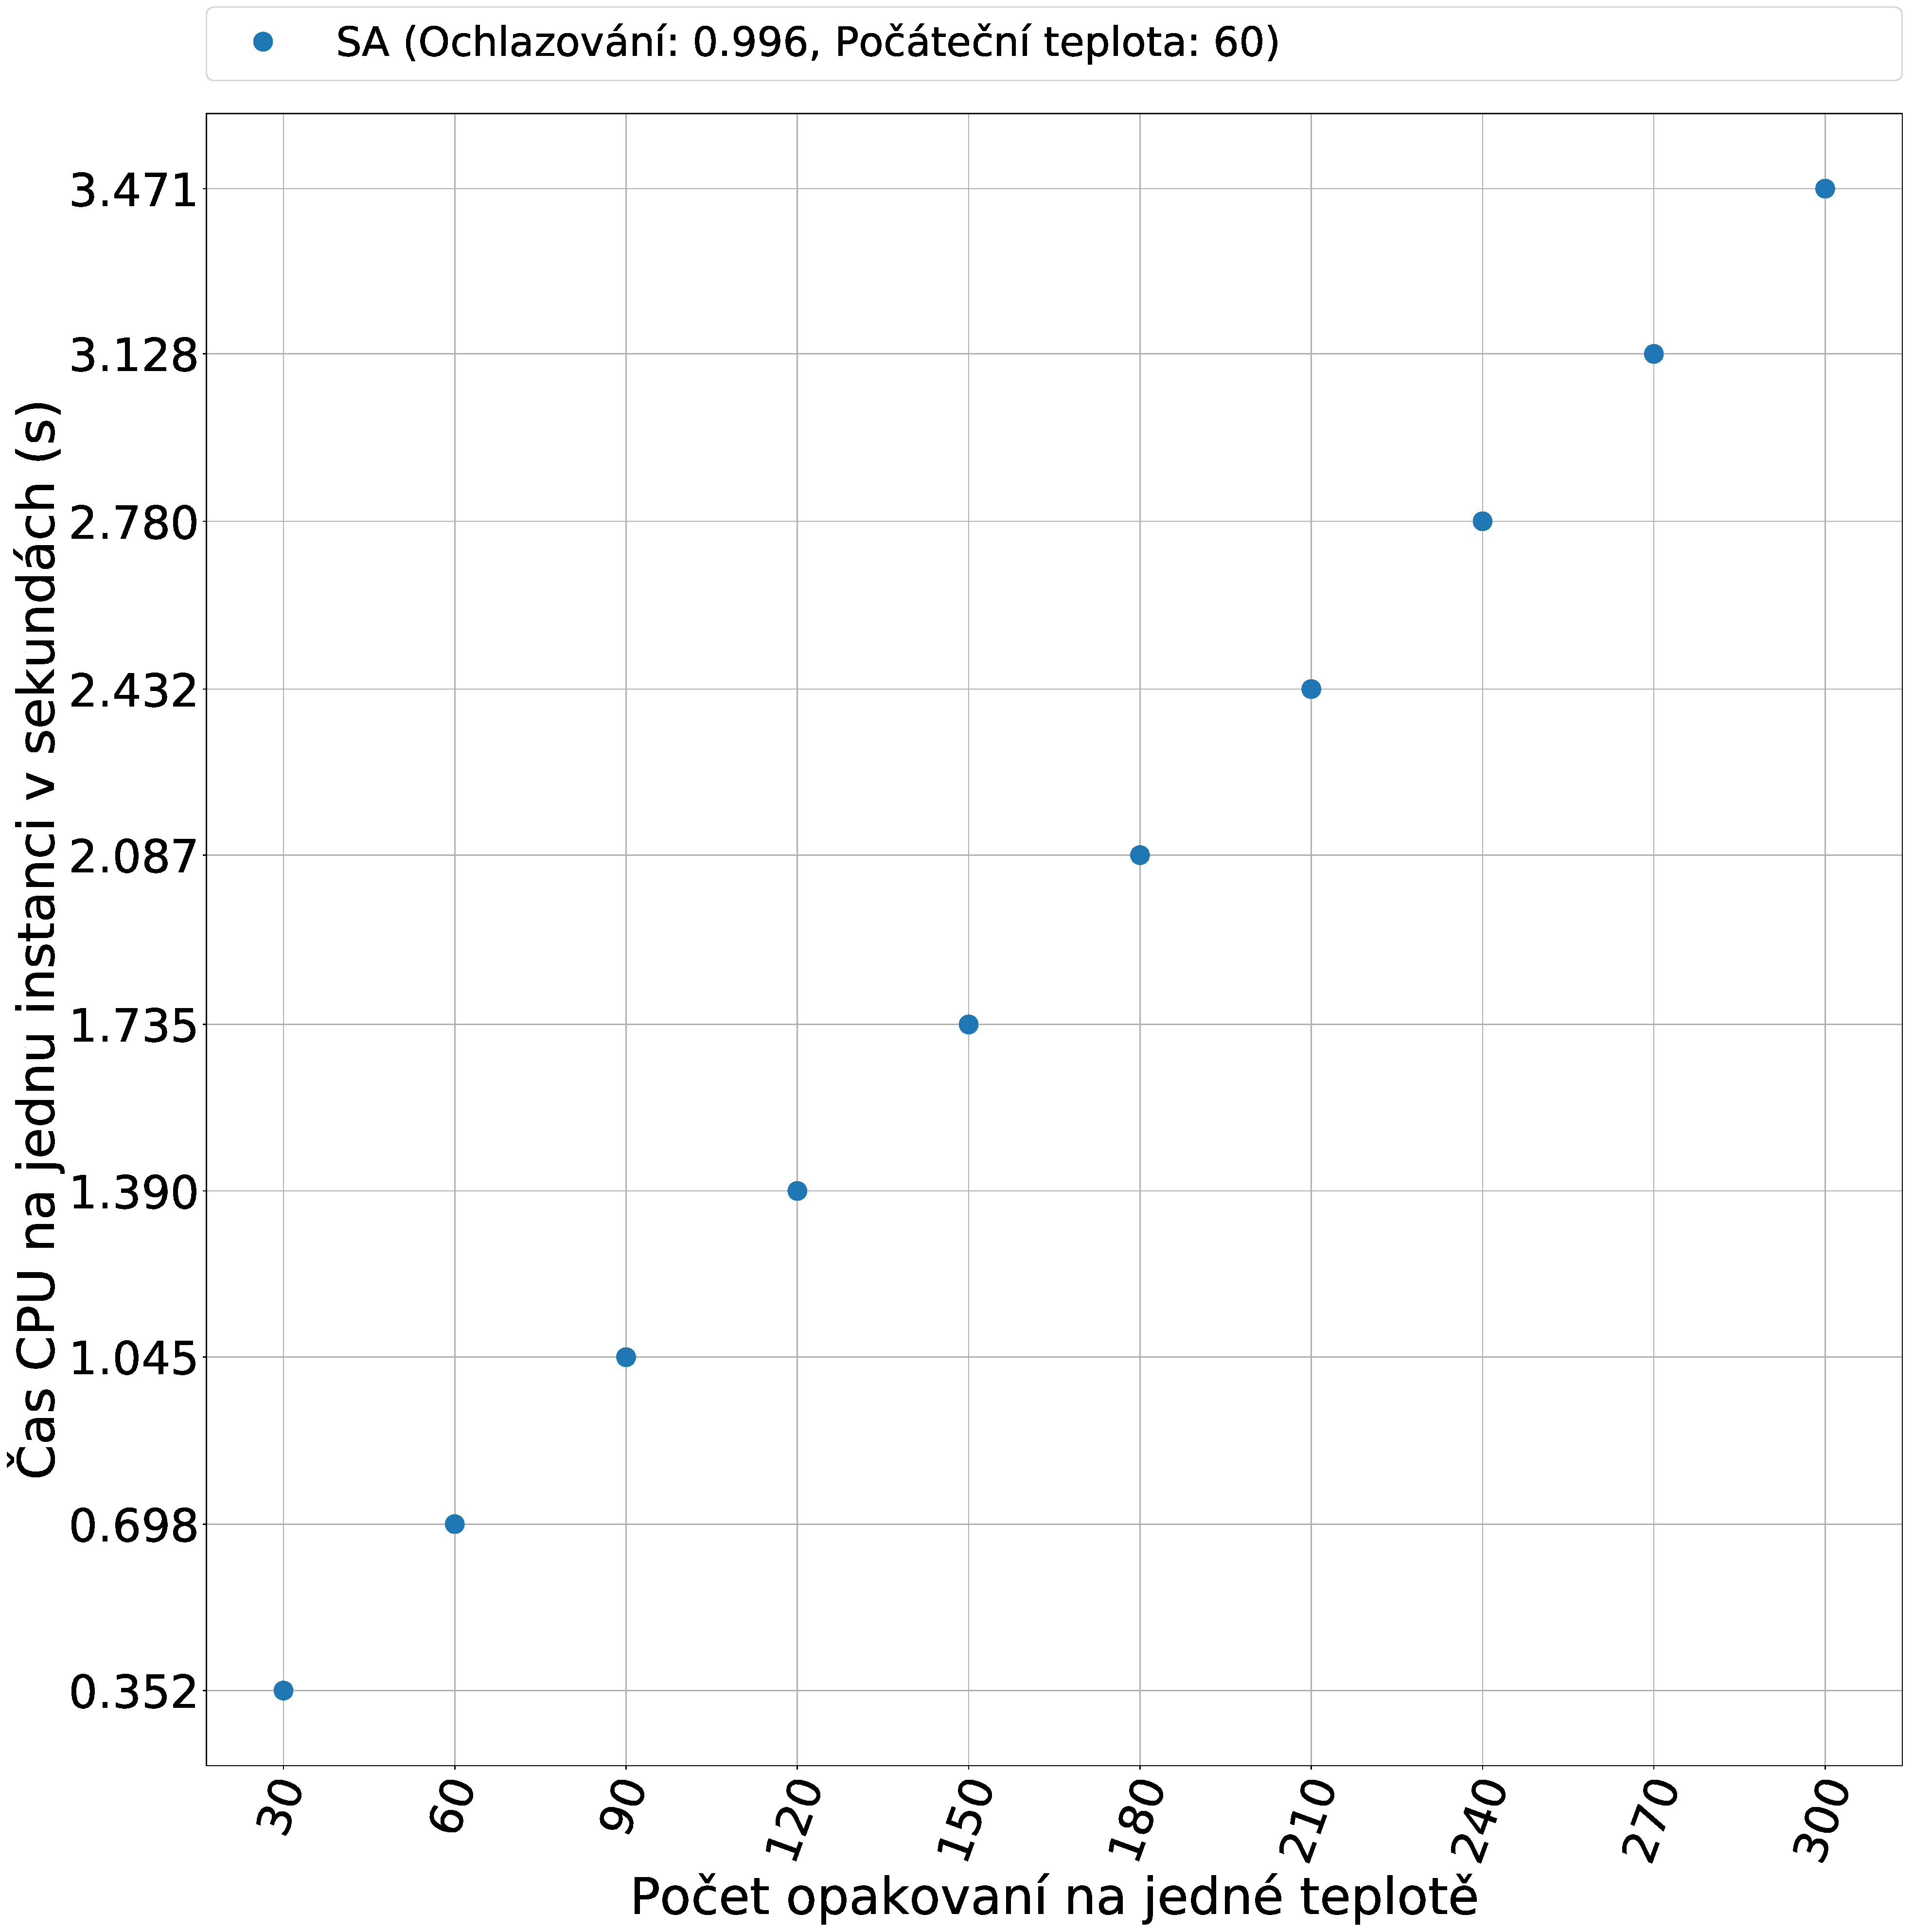
\includegraphics[width=\textwidth]{img/CT.pdf} 
    \end{minipage}
    \\
   \caption{Na levém grafu je závislost relativní chyby na počtu iterací na jedné teplotě. Na pravém grafu je závislost výpočetního času na počtu iterací na jedné teplotě}\label{fig:GVI}
\end{figure} 

\begin{figure}
	\centering
    \begin{minipage}[c]{0.325\textwidth}
        \centering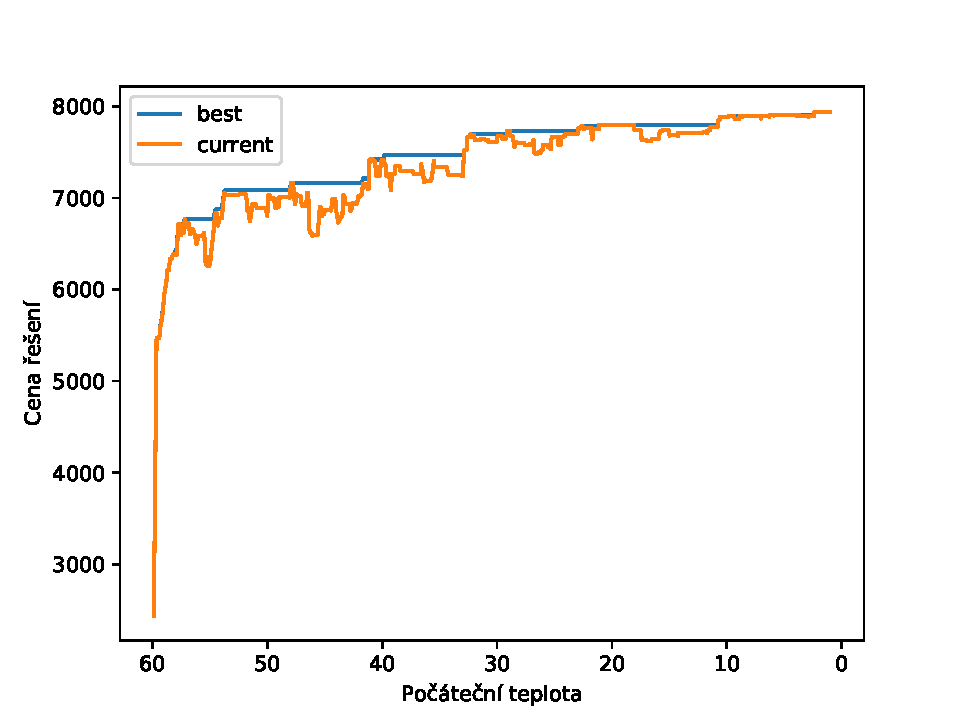
\includegraphics[width=\textwidth]{img/C30.pdf} 
    \end{minipage}
    \begin{minipage}[c]{0.325\textwidth}
        \centering 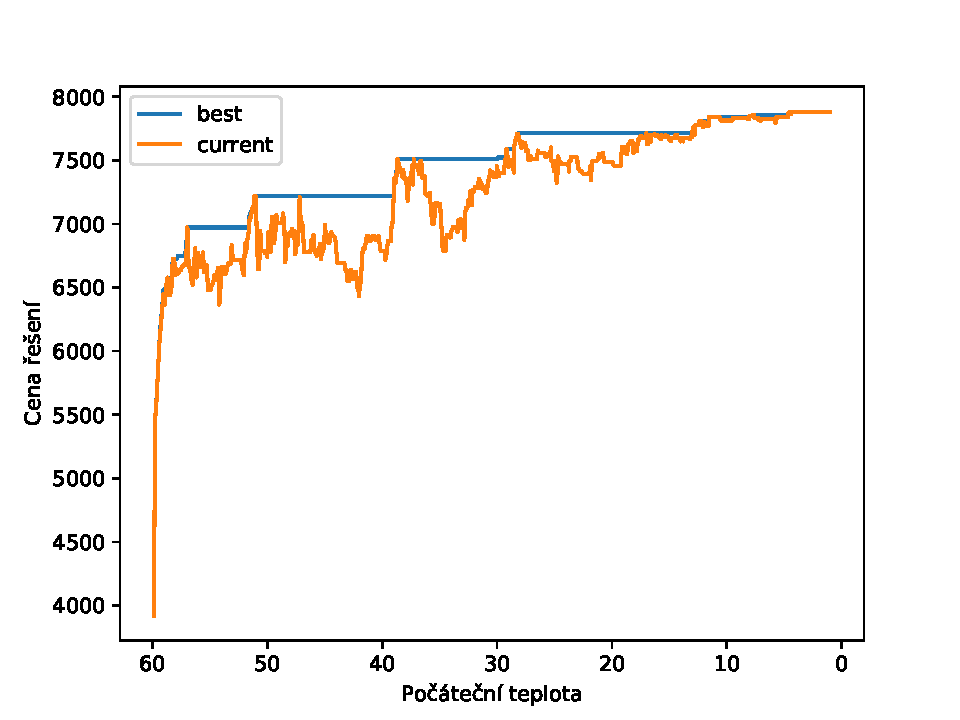
\includegraphics[width=\textwidth]{img/C60.pdf} 
    \end{minipage}
    \begin{minipage}[c]{0.325\textwidth}
        \centering 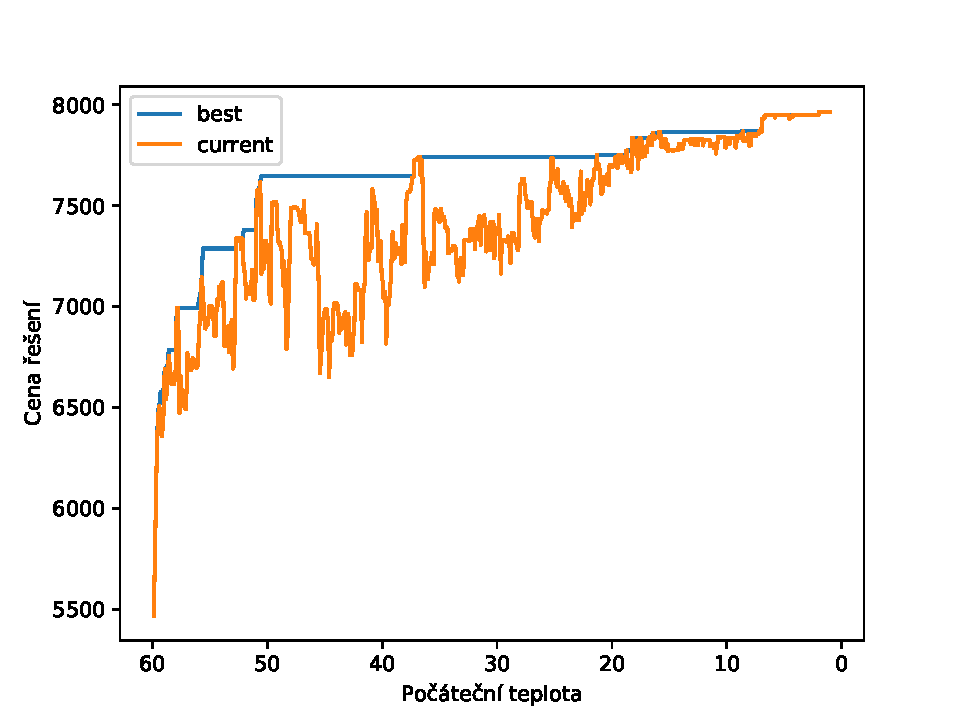
\includegraphics[width=\textwidth]{img/C120.pdf} 
    \end{minipage}
    \\
    \begin{minipage}[c]{0.325\textwidth}
        \centering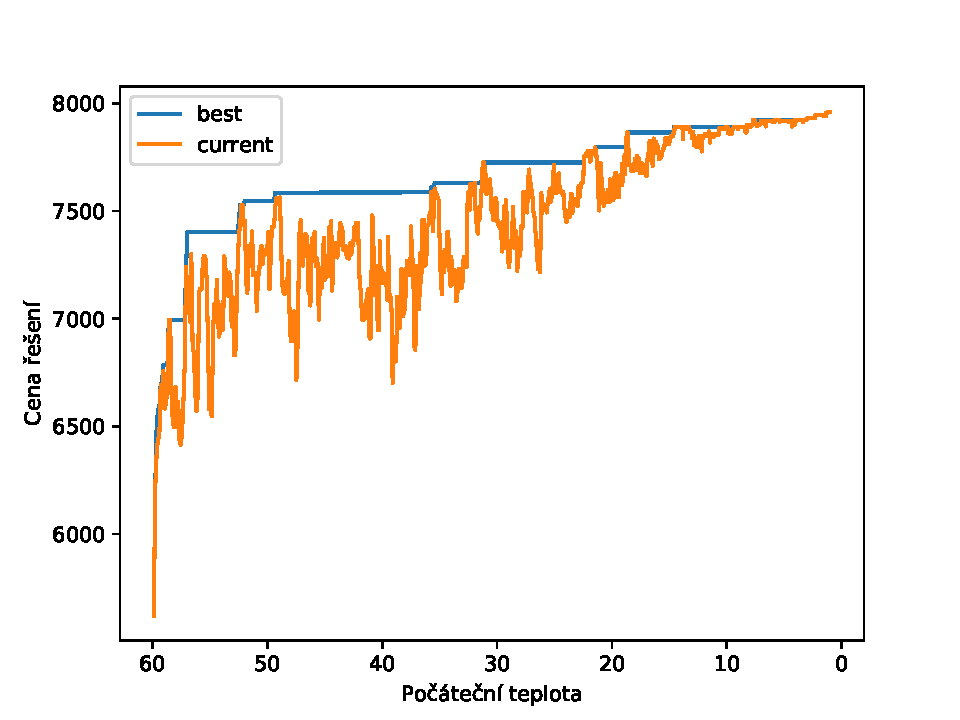
\includegraphics[width=\textwidth]{img/C180.pdf} 
    \end{minipage}
    \begin{minipage}[c]{0.325\textwidth}
        \centering 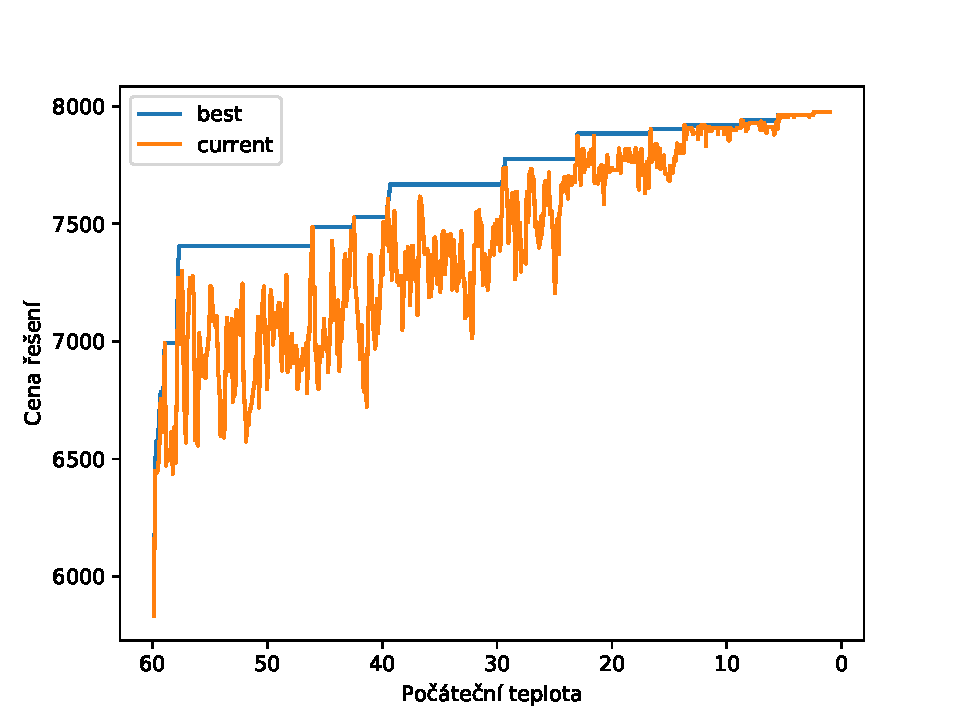
\includegraphics[width=\textwidth]{img/C240.pdf} 
    \end{minipage}
    \begin{minipage}[c]{0.325\textwidth}
        \centering 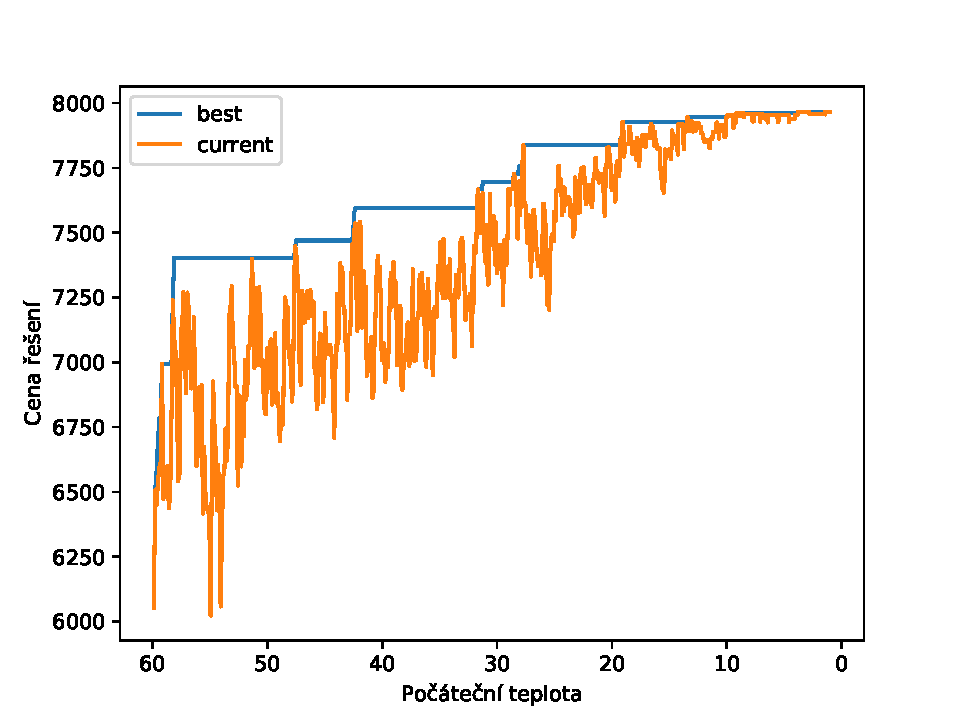
\includegraphics[width=\textwidth]{img/C300.pdf} 
    \end{minipage}
   \caption{Na levém grafu je závislost relativní chyby na počáteční teplotě. Na pravém grafu je závislost výpočetního času na počáteční teplotě}\label{fig:GVI}
\end{figure} 

    
  
\section{Závěr}


\end{document}